%%%%%%%% ICML 2026 two-column format, [preprint] mode for arXiv %%%%%%%%

\documentclass{article}

% Recommended, but optional, packages for figures and better typesetting:
\usepackage{microtype}
\usepackage{graphicx}
\usepackage{booktabs} % for professional tables
% Every figure is regenerated by a script in ../scripts/ (see ../README.md).
\graphicspath{{../figures/}}
\usepackage{tikz}
\usetikzlibrary{decorations.pathreplacing, arrows.meta}

% hyperref makes hyperlinks in the resulting PDF.
% If your build breaks (sometimes temporarily if a hyperlink spans a page)
% please comment out the following usepackage line and replace
% \usepackage{icml2026} with \usepackage[nohyperref]{icml2026} above.
\usepackage{hyperref}

% Attempt to make hyperref and algorithmic work together better:
\newcommand{\theHalgorithm}{\arabic{algorithm}}

% [preprint] shows authors and drops the review-mode footer — arXiv version.
% Swap to plain \usepackage{icml2026} for a blind submission, or
% \usepackage[accepted]{icml2026} for camera-ready.
\usepackage[preprint]{icml2026}

\usepackage{amsmath}
\usepackage{amssymb}
\usepackage{mathtools}
\usepackage{amsthm}

% if you use cleveref..
\usepackage[capitalize,noabbrev]{cleveref}
\usepackage{aliascnt} % lets 'assumption' share the theorem counter yet be named "Assumption" by cleveref

%%%%%%%%%%%%%%%%%%%%%%%%%%%%%%%%
% THEOREMS
%%%%%%%%%%%%%%%%%%%%%%%%%%%%%%%%
\theoremstyle{plain}
\newtheorem{theorem}{Theorem}[section]
\newtheorem{proposition}[theorem]{Proposition}
\newtheorem{lemma}[theorem]{Lemma}
\newtheorem{corollary}[theorem]{Corollary}
\theoremstyle{definition}
\newtheorem{definition}[theorem]{Definition}
% assumption shares the theorem counter (via aliascnt) so numbering continues
% in sequence, but cleveref names it "Assumption" rather than "Theorem".
\newaliascnt{assumption}{theorem}
\newtheorem{assumption}[assumption]{Assumption}
\aliascntresetthe{assumption}
\theoremstyle{remark}
\newtheorem{remark}[theorem]{Remark}
\crefname{assumption}{Assumption}{Assumptions}
\Crefname{assumption}{Assumption}{Assumptions}

% Todonotes is useful during development; disable before submission by
% swapping to \usepackage[disable,textsize=tiny]{todonotes}
\usepackage[textsize=tiny]{todonotes}

% Short form of the title for the running header:
\icmltitlerunning{Can Power Draw Constrain Covert Compute?}

\begin{document}

\twocolumn[
  \icmltitle{Can Power Draw Constrain Covert Compute?}

  \begin{icmlauthorlist}
    \icmlauthor{Tom Kimpson}{unimelb}
    \icmlauthor{Mauricio Baker}{rand}
    \icmlauthor{Emlyn Graham}{tbd}
    \icmlauthor{Anjay Friedman}{rand}
    \icmlauthor{Maximus Rafla}{rand}
    \icmlauthor{Coby Joseph}{rand}
    % Placeholder: further authors to be added here.
  \end{icmlauthorlist}

  \icmlaffiliation{unimelb}{School of Mathematics and Statistics, The University of Melbourne, Parkville, VIC, Australia}
  \icmlaffiliation{rand}{RAND Corporation}
  \icmlaffiliation{tbd}{Affiliation TBD} % TODO: Emlyn Graham's affiliation

  \icmlcorrespondingauthor{Tom Kimpson}{tom.kimpson@unimelb.edu.au}

  % Keywords populate the PDF metadata; they are not shown in the document.
  \icmlkeywords{AI governance, compute verification, power side channel, identifiability, covert compute}

  \vskip 0.3in
]

% Creates the first-column footnote with affiliations; required even if empty.
\printAffiliationsAndNotice{}

\begin{abstract}
Compute governance rests on counting operations: past a threshold, a
training run triggers registration, reporting, and audit obligations.
One channel a verifier can read without trusting the operator's
hardware is an off-chip power meter; the hope is that an energy budget
bounds an operation count. We show exactly when it does. The energy cost
of an operation is unknown and data-dependent, so inverting a power
trace returns a set, not a number; the set's width is a floor on the
covert compute the trace admits.
We derive the floor in closed form from named physical bands and measure
those bands on NVIDIA A100s, evaluating every term inside a single jointly
feasible scenario: one declared format, one covert format, and one
observation window sharing the machine. We construct explicit
same-declaration, same-window cheating witnesses that the meter accepts,
hiding up to four-tenths of a machine of covert work; above these attained
points the model bounds the worst case at one to two machines of the
declared-format capacity ($\beta_{\mathrm{phys}}^{*} = 1.16$ once the
declared precision is checked --- a peak that lies above the utilisation any
single window can hold, and so an upper bound rather than an attained width
--- rising to $1.91$ against a bare meter that cannot even pin the declared
format). The closed form
then prices what each added verifier capability buys and states the
condition each rung rests on: re-execution of the declared work at an
observed operating point brings the floor to a few tenths, under a
stated hardware-transfer assumption. The rungs interlock
--- re-execution pays only at an observed operating point --- and no
capability reaches the covert side, which closes only by assumption on
the adversary. A power-based verification regime can then be designed --- or
rejected --- on numbers rather than on the intuition that joules imply
operations.
\end{abstract}

\section{Introduction}
\label{sec:intro}

%Motivation - what is verification and compute thresholds
As frontier AI systems grow more capable, governance proposals increasingly
turn on \emph{verification}: the ability of an outside party to check what a
compute operator is doing \citep{reuel2025openproblems,baker2025verifying}. One proposed mechanism is a threshold on compute
\citep{sastry2024computing}. Above a specified number of floating-point
operations (FLOP), a training run triggers registration, reporting, or audit
obligations \citep{shavit2023chinchilla,baker2025verifying,heim2024thresholds}. For example, U.S.~Executive Order 14110 required reports on models
trained using more than $10^{26}$ integer or floating-point operations
\citep{whitehouse2023eo14110}, until its revocation in January 2025
\citep{whitehouse2025eo14148}.


%But the prover is not honest
Compute verification policies need to be robust to adversarial operators who do not declare honestly, but instead subvert the threshold by hiding computation. The hardware mechanisms proposed to catch such an operator \citep[e.g. utilisation counters, on-chip clocks, memory telemetry;][]{ogara2025hardware} all read silicon controlled by the operator. Verification methods built on these mechanisms are therefore
conditional on tamper-resistant read paths and attested monitoring firmware
that do not yet exist \citep{ogara2025hardware,rahman2026telemetry}. 


% off-chip analogue sensors
In order to circumvent the reach of the adversarial operator, ``off-chip'' analogue sensors have been suggested as a path forward \citep{baker2025verifying}. These sensors could be retrofitted to existing data centres and physically secured against tampering by the adversary, returning measurements of physical side channels such as power, electromagnetic, acoustic, or thermal emissions.

% prior work: emissions leak workload information
There are reasons for optimism: in non-adversarial settings, physical
emissions are known to leak workload information, from architectures and
hyperparameters down to operand values (\cref{sec:related} surveys this corpus).
But that work fits forward models under cooperative conditions, mapping
known workloads to their emissions. Verification poses the inverse
problem---emissions to workload---against an operator actively trying to
evade the sensor, and the question is how tightly analogue-sensor
measurements can constrain compute in that setting. Of the physical side channels an off-chip sensor could read, we take power
first: it already serves in the governance literature as a coarse proxy for
compute, and it bears the most direct link to computation, since every
operation costs energy and total energy therefore budgets total work. Whether the framework carries to the other channels is open, and we
leave that to future work.

Our contributions:
\begin{itemize}
	\item \textbf{A closed-form identifiability floor.} The covert compute a
	power trace admits is the capacity-clipped
	$\beta_{\mathrm{phys}}(h) = \min[\,S(h),\,(1-h)\,\gamma\,]$, with
	$S(h) = h\,(r_{\mathrm{hi}}^{\mathrm{dec}} -
	r_{\mathrm{lo}}^{\mathrm{dec}})/r_{\mathrm{lo}}^{\mathrm{cov}} + \Delta
	E_0/(r_{\mathrm{lo}}^{\mathrm{cov}} C_{\max})$ the energy-slack index---a
	structural bound that
	precedes statistics: it is what the meter cannot rule out even noiseless
	(\cref{sec:floor}).
	\item \textbf{The bands measured on real silicon.} Factorial,
	single-variable, and dose--response experiments on an A100 ground every
	term: per-format exchange-rate bands (the pooled envelope spans
	$24.8\times$, precision-dominated; the fp16 band alone spans
	$2.0\times$), the descriptive within-device operand
	spread ($w_0 = 1.83$, clock-confounded and priced into no bound), the
	overhead band, and the marginal cost of an added covert
	operation, identified by intervening on the covert dose alone
	($0.51$--$0.76$\,pJ/op one-sided lower limits;
	\cref{sec:empirical-measurements}).
	\item \textbf{The capability ladder, priced.} From the same bands,
	each rung the capacity-clipped worst case
	$\max_h \beta_{\mathrm{phys}}(h)$: $1.91$ (bare meter) $\to 1.16$
	(precision declared and checked, conditional on declared-format
	execution) $\to 0.34$ (declared work re-executed) $\to 0.071$ (covert
	work restricted to useful data), with the measured marginal useful edge
	pricing what covert work is worth doing
	(\cref{sec:decreasing-beta}).
	\item \textbf{A structural asymmetry.} Declarations and re-execution
	narrow only the \emph{declared} band; no channel reaches the covert
	band's floor, which closes only by assumption on the adversary. And the
	rungs interlock: re-execution pays only at an observed operating
	point, so a verifier with power and paperwork but no on-site sensing
	stalls at $\beta_{\mathrm{phys}}^{*} \approx 1$
	(\cref{sec:decreasing-beta}).
\end{itemize}

This paper is organised as follows. \Cref{sec:related} positions the
contribution against prior work; \cref{sec:setup} sets up the problem mathematically.
We then derive a floor on the covert compute a power trace admits, in closed
form from a handful of named physical bands (\cref{sec:floor}). We measure those
bands directly on NVIDIA A100 hardware---one card for the band sweeps,
three more for a cross-device check, together a stand-in for a full
cluster---and
assemble the floor a power meter allows (\cref{sec:empirical-measurements}). Finally we walk that
floor down a capability ladder (\cref{sec:decreasing-beta}): each
capability the verifier gains --- a checked precision declaration, an observed
clock, re-execution of the declared work, an assumption about the adversary's
operands --- moves one edge of the closed form, and the same measured bands
price every rung the verifier can honestly price today. \Cref{sec:discussion} sets out what transfers from device to
facility scale, and what does not.

\section{Related work}
\label{sec:related}

\paragraph{Physical emissions leak workload information.}
In non-adversarial settings, physical emissions let an observer recover
model architectures and hyperparameters
\citep{hu2020deepsniffer,maia2022magnetic,gao2023deeptheft,chaudhuri2025energon},
and software-visible counters and timing let a co-resident process do the
same \citep{naghibijouybari2018rendered,wei2020leaky}. On-node telemetry
and on-chip counters classify workloads
\citep{tang2022supercloud,xu2026wave,gangwal2019cryptomining}, and power
draw betrays anomalous computation \citep{clark2013wattsupdoc} and
running GPU activity \citep{arefin2024hdmi}; a
related body of work characterises power draw for GPUs and data centres
\citep{patel2023polca,choukse2025power,latif2025power}. These are forward
models fitted largely in cooperative conditions---known workload to measured
emission---and they establish the physical premise this paper builds on:
analogue signals carry workload information.

\paragraph{Adversarial detection.}
Closest to our setting, \citet{rahman2026telemetry} evaluate the
\emph{detection} of hidden ML training from zero-overhead telemetry
against an explicitly adversarial operator, across nine GPU models.
Detection asks whether hidden work of a known kind trips a particular
detector; we ask the complementary identification question---how much
compute \emph{any} power-only verifier can bound, whatever detector it
runs---and answer it with a closed-form floor rather than a classifier
benchmark. A detector can raise alarms above the floor; it cannot narrow
the identified set below the physics.

\paragraph{Verification mechanisms and governance.}
Hardware mechanisms for compute verification---utilisation counters,
on-chip clocks, memory telemetry---read silicon the operator controls,
and so are conditional on tamper-resistant read paths and attested
firmware that do not yet exist \citep{ogara2025hardware,ansari2026hardware}.
Cryptographic
proof-of-training protocols \citep{jia2021proofoflearning,garg2023zkpot}
need the prover's cooperation, and active challenge--response schemes
\citep{monfared2026timing} must run their probes on hardware the
operator controls; an operator can also attempt to restructure its
computation to evade compute-based oversight, though
\citet{seferis2025structuring} argue such structuring is itself
detectable. Off-chip
analogue sensing is proposed precisely to escape this trust dependence
\citep{baker2025verifying}; the governance layer it
would serve sets thresholds and reporting duties in operation counts
\citep{sastry2024computing,shavit2023chinchilla,heim2024thresholds,reuel2025openproblems}.
Our contribution to that programme is the exchange rate between what the
sensor reads and what the threshold counts.

\section{Setup and threat model}
\label{sec:setup}

\subsection{The forward model}
\label{subsec:forward}

Fix an observation window $t \in [0,T]$. Let $F(t)$ be the instantaneous rate
of arithmetic operations [op/s], bounded by the hardware capacity
$F_{\max}$. Each operation costs $r(t)$ joules---the \emph{exchange rate}
[J/op]---and the machine draws an additional non-compute overhead $P_0(t)$
(idle draw, cooling, leakage, I/O). The true instantaneous power is then
affine in the operation rate,
\begin{equation}
	P(t) = r(t)\,F(t) + P_0(t),
	\label{eq:forward}
\end{equation}
and a meter reports only a noisy version of it,
\begin{equation}
	P_{\mathrm{obs}}(t) = P(t) + \eta(t),
	\label{eq:obs}
\end{equation}
with $\eta(t)$ a zero-mean measurement noise the prover cannot forge. The
noise is a measurement limit: being zero-mean, it averages away over
the window and shrinks the longer the verifier watches. Throughout this paper
we therefore assume a perfect meter and work with the clean power $P(t)$; every
floor we derive is a floor on what even a noiseless meter can establish.

The exchange rate $r(t)$ is neither constant nor observed.
Component-level analyses of a 45\,nm process put arithmetic and on-chip
memory access at $0.1$--$20$\,pJ per operation depending on format and
operand locality \citep{horowitz2014computing}, and our device-level measurements on a
modern accelerator span $0.8$--$20$\,pJ/op
(\cref{sec:empirical-measurements}). The energy cost of an operation
depends on the operand values being multiplied
\citep{chandrakasan1992lowpower}, on memory traffic \citep{horowitz2014computing},
and on clock speed and voltage \citep{pallipadi2006ondemand}. We count
\emph{hardware} operations---what the silicon actually executes---rather than
model FLOPs, the algorithmically required operations, and we count them as
\emph{nominal operations} of whichever numeric format runs: a multiply--add
retires two nominal ops whether it executes at fp32 or int8, and integer
multiply--adds are ops, not FLOPs. Every executed operation costs joules, so
the meter sees hardware operations.

Two readings of ``energy per operation'' must not be conflated, and the
floor uses each only where it is valid. The \emph{total quotient} $E/C$ of
a measured window folds the overhead into the rate: at mean rate
$\bar F$, $E/C = \bar r + P_0/\bar F$, with $\bar r$ the compute-only cost
and $P_0/\bar F$ the amortised baseline. The declared side enters the
floor only through the \emph{difference} of its band edges at a common
saturated rate (\cref{eq:cov}); the amortised baseline is then common to
both edges and cancels, so a total quotient is the right estimand there
and the overhead $E_0$ is carried once as its own term. The covert cost,
by contrast, enters as a \emph{denominator}, where no such cancellation
occurs: a defensible floor needs a genuine one-sided \emph{lower} bound on
the \emph{incremental} energy an added covert operation must draw,
$\partial E/\partial C_{\mathrm{cov}}$, with the baseline excluded by
construction. That incremental lower bound---not the affine form of
\cref{eq:forward}---is what the security claim rests on, and
\cref{sec:empirical-measurements} identifies it directly by a
dose--response intervention (Experiment~7) rather than by fitting a global
power--rate curve.

Capacity is format-dependent. The peak rate $F_{\max}$ is not one number but
a property of the executing format: an A100's dense peaks run from
$19.5$\,Top/s at fp32 on the CUDA cores through $156$ at tf32 and $312$ at
fp16/bf16 to $624$\,Top/s at int8 on the tensor cores \citep{nvidia2020a100}. We write $F_{\max}^{\mathrm{dec}}$
for the peak of the declared format, which fixes the capacity normaliser
$C_{\max} = F_{\max}^{\mathrm{dec}}\,T$ used throughout, and
\begin{equation}
	\gamma \;=\; \frac{F_{\max}^{\mathrm{cov}}}{F_{\max}^{\mathrm{dec}}}
	\label{eq:capratio}
\end{equation}
for the capacity ratio of a covert format against the declared one
($\gamma = 2$ for int8 covert work against fp16 declared work on an A100).

Format dependence makes joint feasibility a modelling obligation, not a
detail. Every floor we evaluate for a verifier that has \emph{pinned the
declared format}---the headline and every rung below it---is computed inside a
single jointly feasible scenario: one declared format and one covert format
sharing one observation window. The declared band, the capacity normaliser
$C_{\max}$, and the utilisation $h$ all refer to the same declared format;
the covert cost and the covert peak to the same covert format; and the two
streams time-multiplex the machine, so covert work holds at most the
$(1-h)$ share of resource-time the declared work leaves free. We allow the
prover to switch formats between the two streams at zero cost---the
adversary-favorable direction, since any real switching overhead only
shrinks the covert share. What the model forbids is combining extrema that
no single schedule attains: an honest interpretation priced at one format's
dearest cells is only admissible if that format can execute the declared
work at rate $h\,F_{\max}^{\mathrm{dec}}$ at all, and the headline path in
our analysis code rejects any cross-format combination of extrema by
construction (\cref{sec:empirical-measurements}).

The unconditional bare-meter rung of \cref{subsec:poweronly} is the
deliberate exception, because a bare meter pins no format at all: there both
band edges open to the full hardware envelope while $C_{\max}$ and $h$ stay
the fp16 yardstick. That combination is still admissible under the criterion
above---the honest ceiling is the fp32 rate and fp32 can sustain the
declared rate it implies ($h^{*}C_{\max} = 14.0$\,Top/s against a measured
$17.7$\,Top/s fp32 peak)---but it is a cross-format envelope by intent, not a
single-format scenario, and we flag it as such wherever it is quoted.

\subsection{The threat model}
\label{subsec:threat}

There are two parties. The \emph{prover} is the monitored operator: it controls the
workload, the operand values, the numeric formats, the clocks, and the idle
states of the machine, and it may wish to run compute it does not declare.
The \emph{verifier} is the inspecting party: it reads $P_{\mathrm{obs}}$ from
an off-chip meter it trusts, and it never sees $r$, $F$, or $P_0$ separately.
The prover declares a workload of $C_{\mathrm{dec}}$ operations. The verifier wants to know if  $C_{\mathrm{dec}}$ is consistent with $P_{\mathrm{obs}}$. The verifier makes two assumptions:
\begin{assumption}[Trusted meter]
\label{ass:meter}
The power trace cannot be forged: $P_{\mathrm{obs}}$ differs from the true
draw $P$ only by zero-mean noise, which we set to zero throughout.
\end{assumption}

\begin{assumption}[Trusted declaration]
\label{ass:declaration}
The declared computation really ran: the smallest total consistent with the
window is $C_{\mathrm{dec}}$ itself. A power meter cannot by itself confirm
this; independently checking that the declared work ran is a separate
verification problem---the domain of proof-of-learning and zero-knowledge
proof-of-training protocols \citep{jia2021proofoflearning,garg2023zkpot}.
\end{assumption}
Everything else---the exchange rate $r(t)$, the overhead $P_0(t)$, and how the
operation rate $F(t)$ splits between declared and covert work---is under the prover's
control and unobserved.

\subsection{The inverse model}
\label{subsec:noninjective}

Define $G$ as the forward map that carries a workload to its power trace,
\begin{equation}
	G : \bigl(F(\cdot),\, r(\cdot),\, P_0(\cdot)\bigr) \;\longmapsto\; P(\cdot),
	\label{eq:operator}
\end{equation}
defined pointwise by \cref{eq:forward}. The verifier faces an inverse
problem: read the power trace and recover the workload that produced it,
i.e.\ invert $G$. But $G$ is \emph{non-injective}. Since $r(\cdot)$ is free
to vary, a low rate spent on much computation draws exactly the same power as
a high rate spent on little. Distinct workloads $(F,r,P_0)$ map to identical
traces, and a many-to-one map has no inverse. Inversion therefore returns a
set, not a point: the identified set $\mathcal{A}(P_{\mathrm{obs}})$
collects every physically admissible workload that reproduces
$P_{\mathrm{obs}}$ (\cref{fig:noninjective}).

The question \emph{``how many operations ran over the window?"} corresponds to one
specific projection of $\mathcal{A}(P_{\mathrm{obs}})$. Define the total
compute
\begin{equation}
	C \;=\; \int_0^T F\,dt \quad [\text{op}].
	\label{eq:totalcompute}
\end{equation}
Reading $C$ off each admissible workload projects the identified set onto the
$C$-axis,
\begin{equation}
	\bigl\{\, C \;:\; (F,r,P_0) \in \mathcal{A}(P_{\mathrm{obs}}) \,\bigr\} \;=\;
	[\,C_{\mathrm{lo}},\, C_{\mathrm{hi}}\,].
	\label{eq:projection}
\end{equation}
We define $\beta$ as the width of that interval, measured against the
machine's peak declared-format capacity $C_{\max} = F_{\max}^{\mathrm{dec}}T$,
\begin{equation}
	\beta \;\equiv\; \frac{C_{\mathrm{hi}} - C_{\mathrm{lo}}}{C_{\max}}.
	\label{eq:betadef}
\end{equation}
Under \cref{ass:declaration} the lower edge is the declaration itself,
$C_{\mathrm{lo}} = C_{\mathrm{dec}}$, and the normaliser $C_{\max} = F_{\max}^{\mathrm{dec}}T$
is the machine's capacity. The interval runs from that honest baseline up to
the most compute the meter cannot rule out, so the upper edge is the declared
work plus the largest covert load a cheater could slip past the meter,
\begin{equation}
	C_{\mathrm{hi}} \;=\; C_{\mathrm{dec}} \;+\; C_{\mathrm{cov}}^{\max}.
	\label{eq:chi}
\end{equation}
Substituting $C_{\mathrm{lo}} = C_{\mathrm{dec}}$ and \cref{eq:chi} into
\cref{eq:betadef} leaves a single unknown,
\begin{equation}
	\beta \;=\; \frac{C_{\mathrm{hi}} - C_{\mathrm{lo}}}{C_{\max}}
	\;=\; \frac{C_{\mathrm{cov}}^{\max}}{C_{\max}}.
	\label{eq:beta-reduced}
\end{equation}
The width $C_{\mathrm{hi}} - C_{\mathrm{dec}} = C_{\mathrm{cov}}^{\max}$ is
exactly the covert operations a cheater could hide. A wider interval means a larger
$\beta$ and more room for undeclared work; $\beta \gg 1$ means the ambiguity
exceeds the entire machine.

Note that $\beta$ is a floor, not a measurement error. It is the ambiguity that survives a perfect meter: because distinct workloads draw identical
power, no reading of the trace can tell them apart because the data hold no information that separates them. Averaging, longer observation, and better estimators all fight measurement noise, and none of them lowers $\beta$.

\begin{figure*}[t]
	\centering
	\begin{tikzpicture}[>=Stealth, line join=round, line cap=round]

		% ================= (a) two admissible workloads =================
		\begin{scope}[shift={(0,0)}]
			\draw[->] (0,0.55) -- (3.1,0.55) node[right] {\scriptsize $t$};
			\draw[->] (0,0.55) -- (0,2.9) node[above] {\scriptsize $F$};
			\draw[->] (2.9,0.55) -- (2.9,2.9) node[above] {\scriptsize $r$};
			\draw[teal!60!black] (0.15,2.45) -- (2.8,2.45);
			\draw[teal!60!black, dashed] plot[smooth, tension=0.7] coordinates
			{(0.15,0.72) (0.6,1.0) (1.1,1.42) (1.5,1.6) (1.9,1.45) (2.4,1.08) (2.8,0.82)};
			\draw[orange!85!black] (0.15,1.05) -- (2.8,1.05);
			\draw[orange!85!black, dashed] plot[smooth, tension=0.7] coordinates
			{(0.15,0.8) (0.6,1.3) (1.1,2.08) (1.5,2.4) (1.9,2.12) (2.4,1.45) (2.8,0.98)};
			\node[teal!60!black, anchor=south, inner sep=0.5pt] at (2.45,2.46) {\scriptsize $r_A$};
			\node[orange!85!black, anchor=north, inner sep=0.5pt] at (2.45,1.04) {\scriptsize $r_B$};
			\node[teal!60!black, anchor=east, inner sep=1pt] at (0.95,1.62) {\scriptsize $F_A$};
			\node[orange!85!black, anchor=south east, inner sep=0.5pt] at (1.25,2.42) {\scriptsize $F_B$};
			\node[anchor=north] at (1.5,0.35) {\footnotesize (a) two workloads};
		\end{scope}

		\draw[->, thick] (3.25,1.7) -- (4.35,1.7);
		\node[anchor=south, inner sep=1pt] at (3.8,1.78) {\scriptsize $G$};
		\node[anchor=north, inner sep=1pt] at (3.8,1.62) {\scriptsize many$\,\to\,$one};

		% ================= (b) one power trace =================
		\begin{scope}[shift={(4.55,0)}]
			\draw[->] (0,0.55) -- (3.1,0.55) node[right] {\scriptsize $t$};
			\draw[->] (0,0.55) -- (0,2.9) node[above] {\scriptsize $P$};
			\draw[thick, blue!55!black] plot[smooth, tension=0.7] coordinates
			{(0.15,1.2) (0.5,1.5) (0.85,2.05) (1.2,1.85) (1.55,2.3)
				(1.9,2.05) (2.25,2.2) (2.6,1.6) (2.95,1.25)};
			\node[blue!55!black, anchor=south west] at (0.05,2.35) {\scriptsize $P_{\mathrm{obs}}(t)$};
			\node[anchor=north] at (1.5,0.35) {\footnotesize (b) one trace};
		\end{scope}

		\draw[->, thick] (7.8,1.7) -- (8.9,1.7);
		\node[anchor=south, inner sep=1pt] at (8.35,1.78) {\scriptsize invert};
		\node[anchor=north, inner sep=1pt] at (8.35,1.62) {\scriptsize set-valued};

		% ================= (c) identified set = constant-energy arc =================
		\begin{scope}[shift={(9.35,0)}]
			\draw[->] (0,0.55) -- (4.7,0.55) node[right] {\scriptsize $C$};
			\draw[->] (0,0.55) -- (0,3.0) node[above] {\scriptsize $\bar r$};
			\draw[line width=6pt, gray!18, line cap=round, smooth, samples=60, domain=1.0:3.9]
			plot (\x,{1.2776/\x+0.9724});
			\draw[gray!75!black, thick, smooth, samples=60, domain=1.0:3.9]
			plot (\x,{1.2776/\x+0.9724});
			\node[anchor=south west, inner sep=1pt] at (1.5,1.92) {\scriptsize $\bar r\,C=E_c$};
			\node[anchor=south] at (2.95,2.5) {\footnotesize $\mathcal{A}(P_{\mathrm{obs}})$};
			\fill[gray!55] (2.0,1.611) circle (0.9pt);
			\fill[gray!55] (3.0,1.398) circle (0.9pt);
			\fill[teal!60!black]   (1.0,2.25) circle (1.5pt) node[above, inner sep=2.5pt] {\scriptsize $A$};
			\fill[orange!85!black] (3.9,1.3)  circle (1.5pt) node[above right, inner sep=1pt] {\scriptsize $B$};
			\draw[dashed, teal!60!black]   (1.0,2.25) -- (0,2.25);
			\draw[dashed, orange!85!black] (3.9,1.3)  -- (0,1.3);
			\fill (0,2.25) circle (1.0pt) node[left=1pt] {\scriptsize $r_{\mathrm{hi}}$};
			\fill (0,1.3)  circle (1.0pt) node[left=1pt] {\scriptsize $r_{\mathrm{lo}}$};
			\draw[dashed, teal!60!black]   (1.0,2.25) -- (1.0,0.55);
			\draw[dashed, orange!85!black] (3.9,1.3)  -- (3.9,0.55);
			\fill (1.0,0.55) circle (1.2pt) node[below=2pt] {\scriptsize $C_{\mathrm{lo}}$};
			\fill (3.9,0.55) circle (1.2pt) node[below=2pt] {\scriptsize $C_{\mathrm{hi}}$};
			\draw[decorate, decoration={brace, amplitude=5pt, mirror}]
			(1.0,0.10) -- (3.9,0.10) node[midway, below=6pt] {$\beta\,C_{\max}$};
			\node[anchor=north] at (2.0,-0.95) {\footnotesize (c) identified set};
		\end{scope}

	\end{tikzpicture}
	\caption{Non-injectivity of the forward map. (a)~Two workloads ($A$
		little compute at a high rate, $B$ much compute at a low rate) whose
		products $rF$ coincide, so (b)~they drive the identical power trace.
		(c)~Inverting recovers only the set of consistent explanations
		$\mathcal{A}(P_{\mathrm{obs}})$: the rate band
		$[r_{\mathrm{lo}},r_{\mathrm{hi}}]$ cuts the constant-energy arc
		$A$--$B$, whose projection onto the $C$-axis spans
		$[C_{\mathrm{lo}},C_{\mathrm{hi}}]$; relative to capacity that width is
		the floor $\beta$. The faint
		ribbon is meter noise (ignored in this work). Each rate is drawn
		constant only for clarity; in reality $r(t)$ varies in time. This does
		not matter for a question about total operations, which depends on $r(t)$
		only through its op-weighted mean $\bar r = E_c/C$ (compute energy
		$E_c = \int_0^T rF\,dt$ over total operations $C$). That mean is panel (c)'s
		vertical axis, so letting $r(t)$ vary leaves the picture unchanged.}
	\label{fig:noninjective}
\end{figure*}

\section{Derivation of \texorpdfstring{$\beta$}{beta}}
\label{sec:floor}

We now derive a closed form for $\beta$. The derivation is straightforward: integrate the forward model over the window, split the total energy into declared,
covert, and overhead pieces, and ask how large the covert piece can grow
before the total stops looking honest. We work with the integrated trace (i.e. the total energy) rather than the resolved time series. Treating power as affine in the operation rate (\cref{eq:forward}) lets its integral depend on the workload only through time-integrated quantities. This is a modelling assumption; \cref{rmk:incremental} shows that the security bound needs only a weaker one-sided condition on the \emph{incremental} covert cost---measured directly and found near-perfectly linear in \cref{fig:marginal-dose}---with the affine map recovered as the special case that also fixes the closed form.

\subsection{How much compute can hide?}
\label{subsec:derivation}

Integrating the forward model \cref{eq:forward} over $[0,T]$, the left-hand
side is the total energy the meter reports and the right-hand side falls
into two pieces,
\begin{equation}
	E \;=\; \underbrace{\int_0^T r(t)\,F(t)\,dt}_{\text{compute energy } E_c}
	\;+\; \underbrace{\int_0^T P_0(t)\,dt}_{\text{overhead } E_0}.
	\label{eq:integrated}
\end{equation}
The overhead $E_0$ is a nuisance the verifier knows only within a band
$E_0 \in [E_{0,\mathrm{lo}}, E_{0,\mathrm{hi}}]$. We do not ``subtract
off'' a known baseline: the prover controls fans, clocks, and idle states,
so a known-and-removed $P_0$ would hand it a hiding channel.

The compute energy $E_c$ splits into a declared block and a covert block,
\begin{equation}
	\int_0^T r F\,dt \;=\;
	\underbrace{\int_0^T r^{\mathrm{dec}}\,F_{\mathrm{dec}}\,dt}_{\text{declared}} \;+\;
	\underbrace{\int_0^T r^{\mathrm{cov}}\,F_{\mathrm{cov}}\,dt}_{\text{covert}}.
	\label{eq:dec-cov-split}
\end{equation}
The declared block runs $C_{\mathrm{dec}} = \int_0^T F_{\mathrm{dec}}\,dt$
operations, taken known, and the covert block runs the excess
$C_{\mathrm{cov}} = C - C_{\mathrm{dec}}$; this is the compute we are trying
to bound. Write each block's energy as its operation count times a single mean
cost per operation, i.e.\ the op-weighted averages
\begin{equation}
	\bar r^{\,i} \equiv \frac{1}{C_{i}}\int_0^T r^{i}(t)\,F_{i}(t)\,dt
	\;=\; \int_0^T r^{i}(t)\,\frac{F_{i}(t)}{C_{i}}\,dt,
	\label{eq:barr}
\end{equation}
for $i \in \{\mathrm{dec},\,\mathrm{cov}\}$. The second form makes the
averaging explicit: the weight $F_{i}(t)\,dt/C_{i}$ is the fraction of the
block's operations that run in $[t, t+dt]$; it is nonnegative and integrates to
one. The machine therefore draws
\begin{equation}
	E \;=\; \underbrace{\bar r^{\mathrm{dec}}\, C_{\mathrm{dec}}}_{\text{declared work}}
	\;+\; \underbrace{\bar r^{\mathrm{cov}}\, C_{\mathrm{cov}}}_{\text{covert work}}
	\;+\; \underbrace{E_0}_{\text{overhead}},
	\label{eq:cheaterbudget}
\end{equation}
and the verifier sees only $E$.

Both blocks run on the same silicon, so both mean costs are bounded by the
\emph{same} physical envelope $[r_{\mathrm{lo}}, r_{\mathrm{hi}}]$, the
hardware's full range of energy per operation. We nonetheless track them on separate
labels,
$\bar r^{\mathrm{dec}} \in [r_{\mathrm{lo}}^{\mathrm{dec}}, r_{\mathrm{hi}}^{\mathrm{dec}}]$
and
$\bar r^{\mathrm{cov}} \in [r_{\mathrm{lo}}^{\mathrm{cov}}, r_{\mathrm{hi}}^{\mathrm{cov}}]$,
because a verifier with channels beyond the meter may come to know more about
one than the other; with only a power meter the two coincide with that common
envelope.

The verifier raises no alarm so long as the measured total is explainable by
honest declared work at some admissible rate and overhead. The most an
honest run could ever draw is the declared work at the top of its band, on
top of the highest overhead,
\begin{equation}
	E \;\le\; r_{\mathrm{hi}}^{\mathrm{dec}}\,C_{\mathrm{dec}} \;+\; E_{0,\mathrm{hi}}.
	\label{eq:noalarm}
\end{equation}
The test is deliberately one-sided: covert work can only \emph{add} energy, so
a draw is suspicious only when the total runs \emph{high}. A symmetric lower
alarm would flag \emph{under}-delivery---drawing too little to be the declared
work---which is outside the covert-compute threat model, so no lower bound is
imposed (\cref{prop:estimands}(ii)).
Substituting the budget \cref{eq:cheaterbudget} into the no-alarm condition
\cref{eq:noalarm} and rearranging,
\begin{equation}
	C_{\mathrm{cov}}
	\;\le\; \frac{\bigl(r_{\mathrm{hi}}^{\mathrm{dec}} - \bar r^{\mathrm{dec}}\bigr)\,C_{\mathrm{dec}}
	          \;+\; \bigl(E_{0,\mathrm{hi}} - E_0\bigr)}{\bar r^{\mathrm{cov}}}.
	\label{eq:cov}
\end{equation}
A cheater now pushes every free choice on the right-hand side to its limit:
\begin{itemize}
	\item \emph{Run the declared work cheaply,}
	$\bar r^{\mathrm{dec}} \to r_{\mathrm{lo}}^{\mathrm{dec}}$. The verifier
	cannot tell an expensive declared run from a cheap one, so it must allow
	the draw all the way up to $r_{\mathrm{hi}}^{\mathrm{dec}}\,C_{\mathrm{dec}}$;
	the gap
	$(r_{\mathrm{hi}}^{\mathrm{dec}} - r_{\mathrm{lo}}^{\mathrm{dec}})\,C_{\mathrm{dec}}$
	is free energy the prover spends covertly while the total still reads as
	honest work.
	\item \emph{Idle the overhead,} $E_0 \to E_{0,\mathrm{lo}}$, freeing the
	full band width $\Delta E_0 = E_{0,\mathrm{hi}} - E_{0,\mathrm{lo}}$.
	\item \emph{Run the covert work cheaply,}
	$\bar r^{\mathrm{cov}} \to r_{\mathrm{lo}}^{\mathrm{cov}}$, so each hidden
	operation costs as little as the hardware allows.
\end{itemize}
At those values \cref{eq:cov} attains its maximum, the largest covert load
the trace admits,
\begin{equation}
	C_{\mathrm{cov}}^{\max} \;=\;
	\frac{\bigl(r_{\mathrm{hi}}^{\mathrm{dec}} - r_{\mathrm{lo}}^{\mathrm{dec}}\bigr)\,C_{\mathrm{dec}}
	      \;+\; \Delta E_0}{r_{\mathrm{lo}}^{\mathrm{cov}}}.
	\label{eq:covmax}
\end{equation}
Dividing by $C_{\max}$ and writing the declared
\emph{hardware utilisation}
$h = C_{\mathrm{dec}}/C_{\max}$ (the fraction of
the machine's declared-format capacity the declared work occupies), the
energy budget alone caps the covert load at what we call the
\emph{energy-slack index},
\begin{equation}
\;S(h) \;=\; h\,
		\frac{r_{\mathrm{hi}}^{\mathrm{dec}} - r_{\mathrm{lo}}^{\mathrm{dec}}}{r_{\mathrm{lo}}^{\mathrm{cov}}}
		\;+\; \frac{\Delta E_0}{r_{\mathrm{lo}}^{\mathrm{cov}}\,C_{\max}}\,.\;
	\label{eq:beta}
\end{equation}
Pedagogically, Equation \eqref{eq:beta} describes (how much honest work there is) $\times$ (how uncertain its
per-operation cost is), divided by (how cheaply covert work can run), plus a
smaller slack from the overhead band. The first term grows with the
declared-band width and with the declared utilisation: more legitimate work
offers more cover. The second term is the overhead's contribution: joules
the prover frees by idling overhead that the verifier must still allow for.

Note the asymmetry between the numerator and denominator of \cref{eq:beta}.
Declarations and re-execution can narrow the declared band width
$r_{\mathrm{hi}}^{\mathrm{dec}} - r_{\mathrm{lo}}^{\mathrm{dec}}$ in the
numerator, but no declaration reaches the covert floor
$r_{\mathrm{lo}}^{\mathrm{cov}}$ in the denominator; only hardware-wide
observables (clock, voltage) can raise $r_{\mathrm{lo}}^{\mathrm{cov}}$.

\begin{remark}[What the bound actually requires of the measurements]
\label{rmk:incremental}
Two roles, two estimands. The declared edges enter \cref{eq:covmax} only
through their \emph{difference} $r_{\mathrm{hi}}^{\mathrm{dec}} -
r_{\mathrm{lo}}^{\mathrm{dec}}$ at a common saturated rate, so any baseline
amortised equally into both edges cancels and a measured total quotient
$E/C$ is the correct estimand for the numerator (the overhead enters once,
separately, as $\Delta E_0$). The covert cost enters as the
\emph{denominator} $r_{\mathrm{lo}}^{\mathrm{cov}}$, where nothing cancels:
the bound is a valid security guarantee only if $r_{\mathrm{lo}}^{\mathrm{cov}}$
is a genuine one-sided \emph{lower} bound on the \emph{incremental} covert
energy, $g_x(F_{\mathrm{dec}}, F_{\mathrm{cov}}) - g_x(F_{\mathrm{dec}}, 0)
\ge r_{\mathrm{lo}}^{\mathrm{cov}}\,F_{\mathrm{cov}}$ for every admissible
execution $g_x$. Under only this incremental condition the honest energy
slack of \cref{eq:covmax} still divides by $r_{\mathrm{lo}}^{\mathrm{cov}}$,
so the floor holds without the global affine map of \cref{eq:forward}; the
affine model is the special case
$g_x = P_0 + r^{\mathrm{dec}}F_{\mathrm{dec}} + r^{\mathrm{cov}}F_{\mathrm{cov}}$,
which additionally makes $S(h)$ linear in $h$. We therefore identify
$r_{\mathrm{lo}}^{\mathrm{cov}}$ by a dose--response intervention
(Experiment~7 for the generic int8 edge, Experiment~8 for the useful-operand
edge), not by fitting a power--rate curve; a total-quotient covert edge is
inadmissible here, and every covert edge the bound uses is a marginal dose
slope.
\end{remark}

\subsection{The capacity clip}
\label{subsec:capclip}

The energy budget is not the only physical constraint---and calling
$S(h)$ itself the floor $\beta$ overstates the ambiguity, because covert
work must also \emph{fit on the machine}. The setup already bounds the
operation rate by the executing format's peak (\cref{subsec:forward}), so
however much energy slack the trace leaves, the covert block can never
retire more than the capacity the declared work leaves free. Declared work
occupies a fraction $h$ of the declared-format capacity; the remainder,
executed at the covert format's peak, holds at most
\begin{equation}
	C_{\mathrm{cov}} \;\le\; (1-h)\,\gamma\,C_{\max},
	\label{eq:capclip}
\end{equation}
with $\gamma = F_{\max}^{\mathrm{cov}}/F_{\max}^{\mathrm{dec}}$ the capacity
ratio of \cref{eq:capratio}. We evaluate \cref{eq:capclip} at the
\emph{published peak} capacities rather than the rates our kernels achieve.
This is the adversary-favorable direction and therefore the conservative one
for an upper bound on the ambiguity: peaks give the covert stream more room
than it can really use, so the conceded $\beta_{\mathrm{phys}}$ is larger
than an achieved-rate evaluation would give. On our own measured peaks
($246.9$\,Top/s fp16 and $307.7$\,Top/s int8, so $\gamma = 1.25$ rather than
$2$) the bare-meter rung falls from $1.91$ to $1.22$ and the precision rung
from $1.16$ to $0.91$. \Cref{ass:corners} asks for achieved throughputs when
it certifies that a particular \emph{witness} is realisable in one window,
and the witnesses of \cref{subsec:proposition} are checked that way; the
model bound itself is deliberately evaluated at peaks. The identified-set
width is the smaller of the two constraints,
\begin{equation}
	\;\beta_{\mathrm{phys}}(h) \;=\;
	\min\bigl[\,S(h),\; (1-h)\,\gamma\,\bigr],\;
	\label{eq:betaphys}
\end{equation}
and this, not $S(h)$, is the floor: $\beta = \beta_{\mathrm{phys}}(h)$ in
the sense of \cref{eq:betadef}. The two constraints pull in opposite
directions. The slack $S(h)$ \emph{rises} with $h$---more declared work
offers more cover---while the clip $(1-h)\,\gamma$ \emph{falls}---more
declared work leaves less machine to hide on. At full declared utilisation
the machine is spoken for and $\beta_{\mathrm{phys}}(1) = 0$; at idle there
is capacity but almost no cover. The worst case sits at the crossing,
\begin{equation}
	h^{*} = \frac{\gamma - b}{s + \gamma}, \qquad
	\beta_{\mathrm{phys}}^{*} = \gamma\,\frac{s + b}{s + \gamma},
	\label{eq:betaphysworst}
\end{equation}
writing $S(h) = s\,h + b$ for its slope and intercept. Each side of the
minimum is the binding constraint in its own regime: energy binds for
$h < h^{*}$ (the trace itself caps the covert load), capacity binds for
$h > h^{*}$, and both bind at the crossing. Where the crossing sits is an
empirical question about $s$. On jointly consistent bands---one declared
format's own band over the covert format's marginal cost---the measured
slope is of order one (\cref{sec:empirical-measurements}), so the crossing
falls at intermediate utilisation and the worst case is a fraction of
$\gamma$. The index $S$ retains its meaning as an \emph{energy-only
diagnostic}---$S > 1$ says the energy budget on its own cannot rule out a
machine's worth of covert work---but it is never quoted as the width of
the identified set.

\subsection{The power-only floor}
\label{subsec:poweronly}
A power meter reports total energy and nothing more: to it an operation is an operation, declared or covert, so there is no way
to constrain the declared rate separately from the covert one. The two bands
have no choice but to coincide, both equal to the full hardware envelope:
$r_{\mathrm{hi}}^{\mathrm{dec}} = r_{\mathrm{hi}}$ and
$r_{\mathrm{lo}}^{\mathrm{dec}} = r_{\mathrm{lo}}^{\mathrm{cov}} = r_{\mathrm{lo}}$.
Setting these equal in \cref{eq:beta} collapses the energy-slack index to its
single-band, power-only form
\begin{equation}
	S_{\varnothing}(h) \;=\; h\!\left(\frac{r_{\mathrm{hi}}}{r_{\mathrm{lo}}} - 1\right)
	\;+\; \frac{\Delta E_0}{r_{\mathrm{lo}}\,C_{\max}},
	\label{eq:betabare}
\end{equation}
where the subscript $\varnothing$ denotes the empty set of extra channels:
the meter is all the verifier has. The corresponding power-only floor is its
clip, $\beta_{\mathrm{phys}}(h) = \min[\,S_{\varnothing}(h),\,(1-h)\,\gamma\,]$.
Two limits bracket the first term of \cref{eq:betabare}. First
is \emph{ambiguity}: if the rate is known exactly
($r_{\mathrm{hi}} = r_{\mathrm{lo}}$) the term vanishes, since a pinned
energy budget converts covert joules straight back into operations. Second is
\emph{opportunity}: if the machine is idle
($h = 0$) it vanishes too, with no declared work
to hide beneath. The overhead term, by contrast, needs no declared cover at
all.

\paragraph{A worked example.}
To put a number on the power-only floor, take $C_{\max}=100$ operation-units,
declared work $C_{\mathrm{dec}}=50$, a rate known only to lie in $[1.5, 2.5]$,
and an overhead band $E_0 \in [10, 20]$.
A cheater runs $C=90$ at the efficient end $\bar r = 1.5$ with the overhead
idled to $E_0 = 10$, drawing $E = 1.5 \times 90 + 10 = 145$: exactly
the energy of honest declared work at the expensive end under high overhead,
$2.5 \times 50 + 20 = 145$. No alarm. The verifier cannot separate the
honest $50$ from the true $90$---not for want of statistical power but
structurally: the two hypotheses are energy-degenerate, and no test on the
total can separate them. Of the $40$ covert units, ${\approx}33$ hid under
the rate ambiguity of the declared work (the first term of
\cref{eq:betabare}) and ${\approx}7$ under the overhead band (the second).
In the language of \cref{eq:betadef}: $C_{\mathrm{lo}} = 50$,
$C_{\mathrm{hi}} = 90$, so $\beta = 40/100 = 0.4$. \Cref{eq:betabare}
assembles the same number term by term:
$S_{\varnothing}(0.5) = 0.5\,(2.5/1.5 - 1) + 10/(1.5 \times 100) = 1/3 + 1/15 = 0.4$.
The cheat is also capacity-feasible---the $40$ covert units fit inside the
$(1-h)\,\gamma\,C_{\max} = 50$ units the declared work leaves free (taking
$\gamma = 1$)---so here the clip of \cref{eq:betaphys} is slack and
$\beta_{\mathrm{phys}}(0.5) = 0.4$. Had the slack exceeded $50$ units, the
identified set would have ended at the capacity edge instead: at full
declared utilisation $\beta_{\mathrm{phys}}$ vanishes no matter how wide
the rate band is.

\subsection{What exactly does \texorpdfstring{$\beta$}{beta} bound?}
\label{subsec:proposition}

The derivation above moves through four quantities that are easy to
conflate, so we separate them formally. Throughout, the verifier observes
the total energy $E$, knows the declaration $C_{\mathrm{dec}}$ (hence
$h$), and carries the band knowledge
$\bar r^{\mathrm{dec}} \in [r_{\mathrm{lo}}^{\mathrm{dec}}, r_{\mathrm{hi}}^{\mathrm{dec}}]$,
$\bar r^{\mathrm{cov}} \ge r_{\mathrm{lo}}^{\mathrm{cov}}$,
$E_0 \in [E_{0,\mathrm{lo}}, E_{0,\mathrm{hi}}]$ of
\cref{subsec:derivation}, together with the capacity constraint
\cref{eq:capclip}. The bands are treated as a rectangle: each edge
attainable independently of the others.

\begin{assumption}[Joint feasibility of band corners]
\label{ass:corners}
There exist admissible workloads that attain the cheating corner
$(\bar r^{\mathrm{dec}}, E_0, \bar r^{\mathrm{cov}}) =
(r_{\mathrm{lo}}^{\mathrm{dec}}, E_{0,\mathrm{lo}}, r_{\mathrm{lo}}^{\mathrm{cov}})$
jointly, and under shared constraints: the \emph{same} observation window
$T$, the \emph{same} trusted declared work $C_{\mathrm{dec}}$, one device in
a \emph{common thermal and clock state} whose resource-time the declared and
covert streams multiplex at their \emph{achieved} (not nominal-peak)
throughputs, and the per-format capacities of \cref{eq:capclip}. Without this
the rectangle is an \emph{outer relaxation} of the true feasible set and every
width below is an upper bound rather than an exact width. The corner is not
assumed on faith: we exhibit workloads meeting these constraints and attaining
it up to $h \approx 0.22$ (the \emph{Measured witnesses} below), while above
the busy-time ceiling $h_{\max}$---including the headline $h^{*}$---no single
window realises it and the widths revert to upper bounds.
\end{assumption}

\begin{proposition}[Four estimands]
\label{prop:estimands}
Fix $C_{\mathrm{dec}}$ and the no-alarm rule \cref{eq:noalarm}. Then:
\begin{enumerate}
	\item[(i)] \emph{Identified width, given the observation.} For an
	observed total $E$, the $C$-projection \cref{eq:projection} of the
	identified set has width
	$W(E) = \min\!\bigl[\max\!\bigl(0,\,(E - r_{\mathrm{lo}}^{\mathrm{dec}} C_{\mathrm{dec}}
	- E_{0,\mathrm{lo}})/r_{\mathrm{lo}}^{\mathrm{cov}}\bigr),\;
	(1-h)\,\gamma\,C_{\max}\bigr]$: the covert load the trace cannot rule
	out depends on how much energy was actually drawn. The outer clamp to $0$
	covers observations below the honest lower edge
	$r_{\mathrm{lo}}^{\mathrm{dec}} C_{\mathrm{dec}} + E_{0,\mathrm{lo}}$ (see
	(ii)): there no honest-plus-covert schedule reproduces $E$, the identified
	set is empty, and $W(E)$ is $0$ by convention rather than negative.
	\item[(ii)] \emph{One-sided acceptance region (intentionally permissive).}
	The no-alarm rule \cref{eq:noalarm} accepts exactly the totals
	$E \le r_{\mathrm{hi}}^{\mathrm{dec}} C_{\mathrm{dec}} + E_{0,\mathrm{hi}}$.
	The rule is deliberately permissive: covert work only \emph{adds} energy, so
	the test guards only against draws that run \emph{high} and does not certify
	that every accepted draw is honestly explainable. Accepted draws split in
	two. Those at or above the honest lower edge
	$r_{\mathrm{lo}}^{\mathrm{dec}} C_{\mathrm{dec}} + E_{0,\mathrm{lo}}$
	\emph{are} explainable by honest declared work at some admissible rate and
	overhead; those \emph{below} it are accepted too but are \emph{not}
	honestly explainable---honest work cannot draw that little---so their honest
	identified set is empty ($W(E) = 0$ in (i)). Such under-draws indicate
	\emph{under}-delivery, which lies outside the covert-compute threat model, so
	the rule tolerates them by design rather than imposing a lower alarm. The
	worst-case widths (iii)--(iv) are set at the region's \emph{upper} boundary,
	where the identified set is largest, so the empty lower regime never binds
	them. The modelled decision rule, and the empirical $3\sigma$ rule of
	\cref{sec:empirical-measurements}, are therefore one-sided.
	\item[(iii)] \emph{Worst case over accepted observations.} The largest
	identified width over the acceptance region, in units of $C_{\max}$ and
	ignoring capacity, is attained at the region's top edge and equals the
	energy-slack index: $\sup_E W(E)/C_{\max} = S(h)$ of \cref{eq:beta}.
	\item[(iv)] \emph{Capacity-clipped minimax width.} Restoring
	\cref{eq:capclip}, the worst case becomes
	$\beta_{\mathrm{phys}}(h) = \min[\,S(h),\,(1-h)\,\gamma\,]$ of
	\cref{eq:betaphys}, and the verifier-free headline is its maximum over
	utilisation, $\beta_{\mathrm{phys}}^{*}$ at $h^{*}$
	(\cref{eq:betaphysworst}).
\end{enumerate}
Under \cref{ass:corners} the suprema in (iii) and (iv) are attained;
otherwise they are upper bounds.
\end{proposition}

The proof is the derivation already given: (i)--(ii) restate
\cref{eq:cov,eq:noalarm}; (iii) is the corner argument of
\cref{subsec:derivation} evaluated at the top of the acceptance region;
(iv) intersects with \cref{eq:capclip}. The distinctions matter because
only (i) is a statement about a particular audited window; (iii) and (iv)
are design-time guarantees about what \emph{any} accepted window could
hide. Quoting (iii) as if it were (i) overstates the ambiguity of a
typical window; quoting it without (iv) overstates what physics admits.

\paragraph{Measured witnesses.}
Two measurements bear on the assumptions above
(hardware and protocol in \cref{sec:empirical-measurements}). First, we
witness \cref{ass:corners} directly. On one A100 we ran matched pairs
that hold the trusted declaration and the observation window fixed by
construction: run~A executes $N$ declared fp16 iterations on dear
operands (the $r_{\mathrm{hi}}^{\mathrm{dec}}$ edge) and idles to a
fixed $T = 10$\,s window; run~B executes the \emph{same} $N$ iterations
on cheap operands (the $r_{\mathrm{lo}}^{\mathrm{dec}}$ edge) plus a
covert int8 fill tuned to match A's energy, padded to the same window.
Over eight interleaved repeats at $h = 0.10$, run~A drew
$1291.3 \pm 4.4$\,J and run~B $1279.3 \pm 5.6$\,J, matching to
$|\Delta E|/E = 0.9\%$ while B hid $3.5\times 10^{4}$ covert int8
iterations; the one-sided no-alarm rule of \cref{prop:estimands}(ii), set
three standard deviations above the honest mean, accepted \emph{every}
cheating repeat. Clock locking is denied here as elsewhere, so the arms are
matched by cadence rather than by a held clock: both reach the same
$1410$\,MHz compute clock, and the per-window \emph{median} clock differs
between them only through the idle-pad share, exactly as in Experiment~7.
The asymmetry that remains is conservative. Run~A's dear burst draws
${\approx}500$\,W against run~B's ${\approx}245$\,W and consequently sits at
the card's software power cap, which truncates A's measured honest energy;
since the acceptance threshold is set from A's mean, and the covert dose is
tuned against it, the cap tightens the bar run~B must clear and understates
the covert load the tuner can afford. The
construction holds up to a busy-time ceiling: run~B multiplexes cheap
declared work and roughly two covert operations per declared operation
into one window, so above $h_{\max} \approx 0.24$ its work no longer
fits $T$. We witness the corner at $h = 0.10$, $0.15$, and $0.216$,
where the accepted covert load reaches $0.19$, $0.29$, and $0.41$
machines of declared-format capacity respectively---a measured,
capacity- and time-feasible lower bound on the ambiguity, rising toward
the ceiling. The margin narrows as it rises, and the topmost witness is
the thin one: at $h = 0.216$ the cheating arm's spread is $2.6\times$ the
honest arm's and its dearest repeat ($1969.5$\,J) lands above the honest
arm's dearest ($1964.6$\,J), clearing the $3\sigma$ threshold by $0.86\%$
of the honest mean. The $0.41$ figure should be read as the largest load
we could get accepted, not a comfortable one. Above $h_{\max}$---including the headline
$h^{*} = 0.42$---no single window realises the corner, so there
$\beta_{\mathrm{phys}}$ is an upper bound: the wall-clock budget binds
before the energy budget, and a verifier reading time as well as energy
constrains more than \cref{prop:estimands}, which prices the energy
channel alone. That joint energy--time inversion is future work. Second,
the \emph{transfer gap} behind
re-execution (\cref{sec:decreasing-beta}) is grounded by re-measuring the
band edges on three A100s of the same SKU: every edge agrees to
$2$--$3\%$ across devices, so same-SKU re-execution transfers bands at the
few-per-cent level.

\section{How big is \texorpdfstring{$\beta$}{beta}?}
\label{sec:howbig}

So far the floor is only a pair of formulas---the energy-slack index
\cref{eq:betabare} and its capacity clip \cref{eq:betaphys}; this section asks
how large they actually are. We first analyse the slack's two terms and their
physical drivers (\cref{subsec:factors}), then pin down the value two ways: an
order-of-magnitude estimate from textbook physics (\cref{subsec:envelope}),
and a direct measurement on an NVIDIA A100
(\cref{sec:empirical-measurements}).

\subsection{The two terms}
\label{subsec:factors}

The energy-slack index \cref{eq:betabare} is a sum of two terms: an ambiguity term
$h\,(r_{\mathrm{hi}}/r_{\mathrm{lo}} - 1)$, set by the
spread of the exchange rate, and an overhead term
$\Delta E_0/(r_{\mathrm{lo}}\,C_{\max})$, set by the width of the overhead band.
We take each in turn.

\paragraph{The exchange-rate term.}
Its size is governed by the ratio $r_{\mathrm{hi}}/r_{\mathrm{lo}}$. A chip's
power divides into a dynamic (switching) part and a static part; the exchange
rate comes from the dynamic part, the CMOS switching power
$P_{\mathrm{dyn}} = \alpha C V^2 f$ \citep{chandrakasan1992lowpower}, whose cost
per operation factors into
\begin{equation}
	r \;\approx\; \kappa(\text{precision})\,\cdot\,\alpha(\text{operands})\,\cdot\,
	C_{\mathrm{eff}}(\text{locality},\,\text{kernel})\,\cdot\, V^2.
	\label{eq:cmos}
\end{equation}
\Cref{app:cmos} derives this factorisation; the static part---leakage, cooling,
and idle draw---does not enter $r$ but resurfaces as the overhead term below.
Each factor is set by a different physical scale of the machine
(\cref{fig:exchange-scales}). The numeric-format scale $\kappa$ falls with datapath width at
each precision step (fp32 $\to$ int8), tracking the pJ-scale energy hierarchy of
arithmetic \citep{horowitz2014computing}; the activity factor $\alpha$ is the
data-dependent fraction of transistors that toggle for the given operands; the
effective capacitance $C_{\mathrm{eff}}$ depends on where operands live and which
kernel runs. Less-local operands activate more of the memory hierarchy---storage
arrays and peripheral logic, buffers and interfaces, as well as interconnect---so
their combined dynamic cost is represented by a larger effective switched
capacitance \citep{horowitz2014computing,chatterjee2017architecting}; and $V^2$ is the
capacitor-charging energy of the supply voltage, which DVFS slides along the
voltage--frequency curve \citep{pallipadi2006ondemand}. With the power meter as
the only channel, every one of these factors is unknown to the verifier and
conceded at once.

\begin{figure*}[t]
	\centering
	\begin{tikzpicture}[
		>=Stealth, line join=round, line cap=round,
		panel/.style={draw=black!16, fill=black!1, rounded corners=3pt,
			line width=0.6pt},
		badge/.style={rounded corners=2pt, inner sep=2.5pt,
			font=\footnotesize},
		note/.style={font=\scriptsize, align=center},
		title/.style={font=\footnotesize},
		tiny/.style={font=\tiny},
		mos/.style={font=\tiny, draw=orange!85!black, fill=orange!7,
			rounded corners=1pt, minimum width=0.62cm, minimum height=0.33cm,
			inner sep=1pt},
		logic/.style={font=\scriptsize, draw=blue!55!black, fill=blue!5,
			circle, minimum size=0.42cm, inner sep=0pt},
		fma/.style={font=\tiny, draw=blue!55!black, fill=blue!8,
			rounded corners=1pt, minimum height=0.4cm, inner sep=1.5pt},
		mem/.style={font=\tiny, draw=teal!60!black, fill=teal!4,
			rounded corners=1pt, minimum height=0.4cm, inner sep=1.3pt}]

		% Four equal panels form a physical zoom-out: complementary MOSFETs make
		% logic, logic makes a width-selected FMA, the FMA exchanges operands with
		% the memory hierarchy, and one voltage supply energises the whole path.
		% ============ (1) complementary CMOS switching --- alpha ============
		\begin{scope}[shift={(0,0)}]
			\draw[panel] (0,0.1) rectangle (3.55,4.25);
			\node[title] at (1.775,3.98) {(1) CMOS switch};
			\draw[black!12] (0.18,3.72) -- (3.37,3.72);

			% A deliberately simple CMOS inverter: the complementary devices share
			% their input and output, and drive one effective load capacitance.
			\node[mos] (pmos) at (1.38,3.35) {pMOS};
			\node[mos] (nmos) at (1.38,2.63) {nMOS};
			\draw[orange!85!black, line width=0.65pt]
				(1.38,3.62) -- (pmos)
				(pmos) -- (1.38,2.99) -- (nmos) -- (1.38,2.22);
			\node[tiny, black, anchor=east] at (1.31,3.60) {\(V\)};
			\draw[orange!85!black] (1.23,2.18) -- (1.53,2.18)
				(1.28,2.10) -- (1.48,2.10) (1.33,2.02) -- (1.43,2.02);
			\fill[orange!85!black] (1.38,2.99) circle (1.2pt);
			\draw[->, orange!85!black] (0.35,2.99) -- (0.95,2.99)
				node[tiny, black, midway, above] {input};
			\draw[orange!85!black] (0.95,2.99) -- (0.95,3.35) -- (pmos.west)
				(0.95,2.99) -- (0.95,2.63) -- (nmos.west);
			\draw[orange!85!black] (1.38,2.99) -- (2.42,2.99) -- (2.42,2.82);
			\draw[orange!85!black, line width=0.7pt] (2.27,2.82) -- (2.57,2.82);
			\draw[orange!85!black, line width=0.7pt] (2.27,2.69) -- (2.57,2.69);
			\draw[orange!85!black] (2.42,2.69) -- (2.42,2.22);
			\draw[orange!85!black] (2.27,2.18) -- (2.57,2.18)
				(2.32,2.10) -- (2.52,2.10) (2.37,2.02) -- (2.47,2.02);
			\node[tiny, anchor=west] at (2.62,2.76) {load \(c_i\)};
			\node[tiny, anchor=south] at (2.02,3.02) {output};

			% An operand changes only some of the many cells in a datapath.
			\foreach \x/\c in {0.82/gray!28,1.20/orange!85!black,
				1.58/orange!85!black,1.96/gray!28,2.34/gray!28,2.72/orange!85!black}
				\fill[\c] (\x-0.12,1.52) rectangle (\x+0.12,1.76);
			\node[tiny, text=orange!85!black] at (1.775,1.31)
				{only changing cells charge their loads};
			\node[badge, fill=orange!85!black, text=white] at (1.775,0.88)
				{\(\alpha\)};
			\node[note, text=orange!85!black] at (1.775,0.43)
				{operand-dependent\\toggling fraction};
		\end{scope}

		\draw[->, thick] (3.63,2.36) -- (4.00,2.36);

		% ============ (2) bit-width-selected FMA --- kappa ============
		\begin{scope}[shift={(4.08,0)}]
			\draw[panel] (0,0.1) rectangle (3.55,4.25);
			\node[title] at (1.775,3.98) {(2) FMA datapath};
			\draw[black!12] (0.18,3.72) -- (3.37,3.72);

			% CMOS logic implements a multiplier followed by an accumulator.
			\node[tiny] (ain) at (0.40,3.35) {\(a\)};
			\node[tiny] (bin) at (0.40,2.99) {\(b\)};
			\node[logic] (mul) at (1.30,3.17) {\(\times\)};
			\node[logic] (add) at (2.34,3.17) {\(+\)};
			\node[tiny] (cin) at (1.70,2.75) {\(c\)};
			\draw[->, blue!55!black] (ain) -- (mul);
			\draw[->, blue!55!black] (bin) -- (mul);
			\draw[->, blue!55!black] (mul) -- (add);
			\draw[->, blue!55!black] (cin) -- (add);
			\draw[->, blue!55!black] (add) -- (3.12,3.17)
				node[tiny, black, right] {\(y\)};
			\foreach \x in {1.12,1.29,1.46,2.16,2.33,2.50}
				\fill[orange!85!black]
					(\x-0.035,3.435) rectangle (\x+0.035,3.505);
			\node[tiny, text=orange!85!black] at (1.82,3.58) {networks of CMOS cells};

			% A fixed-width fabric can hold one wide word or several narrow words.
			% The partitions make the numeric encoding and packing explicit.
			\node[tiny, anchor=east] at (0.58,2.40) {fp32};
			\draw[blue!55!black, fill=blue!13] (0.70,2.26) rectangle (3.05,2.54);
			\node[tiny] at (1.875,2.40) {one 32-bit word};
			\node[tiny, anchor=east] at (0.58,1.95) {fp16};
			\foreach \x in {0.70,1.89}
				\draw[blue!55!black, fill=blue!9] (\x,1.81) rectangle (\x+1.16,2.09);
			\node[tiny] at (1.28,1.95) {16};
			\node[tiny] at (2.47,1.95) {16};
			\node[tiny, anchor=east] at (0.58,1.50) {int8};
			\foreach \x in {0.70,1.30,1.90,2.50}
				\draw[blue!55!black, fill=blue!6] (\x,1.36) rectangle (\x+0.55,1.64);
			\foreach \x in {0.975,1.575,2.175,2.775}
				\node[tiny] at (\x,1.50) {8};
			\node[badge, fill=blue!55!black, text=white] at (1.775,0.88)
				{\(\kappa\)};
			\node[note, text=blue!55!black] at (1.775,0.43)
				{format sets gates and\\results per datapath};
		\end{scope}

		\draw[->, thick] (7.71,2.36) -- (8.08,2.36);

		% ============ (3) memory hierarchy and operand path --- C_eff ============
		\begin{scope}[shift={(8.16,0)}]
			\draw[panel] (0,0.1) rectangle (3.55,4.25);
			\node[title] at (1.775,3.98) {(3) memory hierarchy};
			\draw[black!12] (0.18,3.72) -- (3.37,3.72);
			\node[mem, minimum width=0.55cm] (dram) at (0.45,2.87) {DRAM};
			\node[mem, minimum width=0.58cm] (cache) at (1.32,2.87) {cache};
			\node[mem, minimum width=0.48cm] (reg) at (2.18,2.87) {regs};
			\node[fma, minimum width=0.52cm, line width=0.8pt]
				(memfma) at (3.02,2.87) {FMA};
			% A value can enter at any level, but must reach the register/FMA end.
			% Equal line widths avoid implying that remote physical wires are thicker;
			% the chain length instead shows how many hierarchy stages are activated.
			\draw[->, teal!60!black, line width=0.7pt] (dram) -- (cache);
			\draw[->, teal!60!black, line width=0.7pt] (cache) -- (reg);
			\draw[->, teal!60!black, line width=0.7pt] (reg) -- (memfma);
			\node[tiny, text=teal!60!black] at (1.73,3.34)
				{read \(a,b,c\)};
			\draw[<-, teal!60!black, dashed, line width=0.55pt]
				(dram.south) .. controls (1.25,2.12) and (2.60,2.12) .. (memfma.south);
			\node[tiny, text=teal!60!black, fill=black!1, inner sep=1pt]
				at (1.75,2.18) {write result \(y\)};
			\draw[decorate, decoration={brace, amplitude=4pt, mirror}, teal!60!black]
				(0.22,1.82) -- (3.27,1.82);
			\node[tiny, text=teal!60!black, align=center] at (1.745,1.48)
				{more levels crossed \(\Rightarrow\) more circuits\\and capacitance switched};
			\node[badge, fill=teal!60!black, text=white] at (1.775,0.88)
				{\(C_{\mathrm{eff}}\)};
			\node[note, text=teal!60!black] at (1.775,0.43)
				{locality and kernel set\\capacitance per result};
		\end{scope}

		\draw[->, thick] (11.79,2.36) -- (12.16,2.36);

		% ============ (4) one supply across that same path --- V^2 ============
		\begin{scope}[shift={(12.24,0)}]
			\draw[panel] (0,0.1) rectangle (3.55,4.25);
			\node[title] at (1.775,3.98) {(4) voltage domain};
			\draw[black!12] (0.18,3.72) -- (3.37,3.72);
			% The repeated memory--FMA motif makes this panel a containing scale of
			% panel (3), rather than a visually unrelated die cartoon.
			\draw[violet!70!black, fill=violet!2, rounded corners=2.5pt]
				(0.48,1.72) rectangle (3.10,3.60);
			\draw[violet!70!black, line width=1.05pt] (0.75,3.35) -- (2.84,3.35);
			\node[tiny, text=violet!70!black, fill=violet!2, inner sep=1pt,
				anchor=north] at (1.795,3.31) {supply rail};
			\draw[violet!70!black, line width=0.8pt] (0.75,1.95) -- (2.84,1.95);
			\node[tiny, text=violet!70!black, fill=violet!2, inner sep=1pt,
				anchor=north] at (1.795,1.92) {ground rail};
			\node[mem] (diemem) at (1.12,2.55) {cache/regs};
			\node[fma] (diefma) at (2.46,2.55) {FMA};
			\draw[->, teal!60!black] (diemem) -- (diefma);
			\draw[->, violet!70!black] (1.12,3.35) -- (diemem);
			\draw[->, violet!70!black] (2.46,3.35) -- (diefma);
			\draw[violet!70!black] (diemem.south) -- (1.12,1.95);
			\draw[violet!70!black] (diefma.south) -- (2.46,1.95);
			\draw[<->, violet!70!black, line width=0.8pt]
				(0.38,1.95) -- (0.38,3.35);
			\node[tiny, text=violet!70!black, anchor=east] at (0.34,2.65)
				{\(V\)};
			\node[tiny, text=violet!70!black] at (1.79,1.52)
				{DVFS changes every switching cost};
			\node[badge, fill=violet!70!black, text=white] at (1.775,0.88)
				{\(V^2\)};
			\node[note, text=violet!70!black] at (1.775,0.43)
				{energy to charge each\\switched capacitance};
		\end{scope}

		% The structural factors together set capacitance per operation.
		\draw[decorate, decoration={brace, amplitude=5pt, mirror}, black!45]
			(4.25,-0.05) -- (11.55,-0.05);
		\node[font=\scriptsize] at (7.90,-0.50)
			{format and locality set capacitance per operation};

		% ============ assembled equation ============
		\draw[black!20] (0,-0.88) -- (15.79,-0.88);
		\node[font=\normalsize] at (7.895,-1.47)
			{\(r \;=\;
			{\color{blue!55!black}\kappa}\,\cdot\,
			{\color{orange!85!black}\alpha}\,\cdot\,
			{\color{teal!60!black}C_{\mathrm{eff}}}\,\cdot\,
			{\color{violet!70!black}V^2}\)};
		\node[font=\scriptsize, text=gray!60!black] at (7.895,-1.96)
			{\(f\) cancels from the marginal rate; leakage and cooling leave as
			the overhead \(P_0\), not \(r\)};

	\end{tikzpicture}
	\caption{\textbf{The exchange rate, from transistors to the powered die.}
		Each physical scale contributes one factor to the per-operation energy of
		\cref{eq:cmos}. (1)~A complementary pMOS--nMOS inverter charges or discharges
		its effective load \(c_i\) when its input changes; an operand determines
		what fraction \(\alpha\) of all such cells toggle. (2)~Networks of these
		cells implement the multiply and add of an FMA. The numeric format selects
		the word width (and supported packing), changing the logic engaged per
		arithmetic result and hence \(\kappa\). (3)~The FMA reads operands through
		the register--cache--DRAM hierarchy and writes its result back. Traversing
		more of that hierarchy switches additional array and peripheral circuits,
		buffers and interfaces, and interconnect; their combined dynamic cost is
		represented by \(C_{\mathrm{eff}}\). (4)~Within a voltage domain, the supply places
		\(V\) across the arithmetic and interconnect loads, so DVFS contributes
		\(V^2\) per unit capacitance. The
		clock \(f\) cancels from the marginal rate (\cref{eq:rdyn}) and the static
		draw---leakage, cooling---leaves as the overhead \(P_0\), not \(r\).
		Multiplying the factors recovers \cref{eq:cmos}.}
	\label{fig:exchange-scales}
\end{figure*}

\paragraph{The overhead term.}
The overhead $P_0$---idle draw, cooling, leakage, and I/O---admits no comparably
clean factorisation. The exchange rate, though it too varies with the hardware
and its operating point, obeys a single switching law that resolves into a few
factors with bounded ranges; the overhead obeys no such law. It is a
heterogeneous mix of static leakage, cooling control loops, firmware idle states,
and platform I/O, so no single relation fixes the band width $\Delta E_0$ from
first principles. 

\subsection{Back of the envelope}
\label{subsec:envelope}

Taking the factors in order: the precision scale $\kappa$ spans roughly an
order of magnitude from fp32 down to int8 \citep{horowitz2014computing} (our
own sweep in \cref{sec:empirical-measurements} finds $13.7\times$ from fp32
to int8 at dense operands); the
operand activity $\alpha$ adds a data-dependent factor of order two (no
textbook number exists; we measure it directly in
\cref{sec:empirical-measurements}); locality and kernel set
$C_{\mathrm{eff}}$, for which we conservatively count no extra
factor;\footnote{Per access, DRAM costs about a hundred times more than
on-chip memory \citep{horowitz2014computing}, but the per-operation effect is
diluted by the kernel's bytes-per-operation: negligible for a compute-bound
matmul (as \cref{sec:empirical-measurements} finds), though potentially
large for a memory-bound kernel.} and DVFS moves $V^2$ by a factor of about
$1.5$.\footnote{Supply voltages on modern accelerators sit near $1$\,V
\citep{horowitz2014computing} and DVFS moves them by roughly $\pm 10\%$;
energy per operation scales as the ratio squared,
$(1.1/0.9)^2 \approx 1.5$.} Multiplied, the full hardware ratio
$r_{\mathrm{hi}}/r_{\mathrm{lo}}$ sits conservatively in the tens---but
that span crosses numeric formats, and no single declared workload can be
honestly explained at one format's dearest cells while its capacity is
priced at another's (\cref{subsec:forward}). Within one declared format the
precision factor drops out, leaving operands and DVFS: a jointly feasible
declared band of a factor $2$--$3$, so the slack slope $s$ is of order one
and the ambiguity term reaches, not dwarfs, one machine. The overhead term,
which we cannot fix from first principles (\cref{subsec:factors}), is
additive and only raises the slack. On paper, then, energy binds at low
utilisation, the capacity clip of \cref{eq:betaphys} takes over at high
utilisation, and the worst-case floor sits at a substantial fraction of
the machine---up to about its declared-format capacity as a model bound.
A bare power meter certifies little about how many operations ran. We put
numbers on this next by direct measurement.

\subsection{Measurement on an NVIDIA A100}
\label{sec:empirical-measurements}
We now turn the CMOS factorisation of \cref{eq:cmos} into a measurement
plan. Its factors do not enter \cref{eq:betabare} separately. Dividing
dynamic switching power by operation rate cancels the clock frequency and leaves
$\kappa$, $\alpha$, $C_{\mathrm{eff}}$, and $V^2$ to determine the dynamic
energy per operation $r$; the range they allow is summarised by the exchange-rate
edges $r_{\mathrm{hi}}$ and $r_{\mathrm{lo}}$. Experiment~1 sweeps precision
($\kappa$) and locality ($C_{\mathrm{eff}}$) to find the observed ceiling;
Experiment~2 sweeps operand activity ($\alpha$) and takes its cheapest point
as the observed floor. The platform did not expose voltage control, so we
could not sweep $V^2$; we record the governor-selected clock as
operating-point metadata instead. The static component of the power omitted by \cref{eq:cmos} returns as the intercept $P_0$ of the affine power law;
Experiment~3 measures the width of that intercept band and hence
$\Delta E_0$ over the observation window. The three experiments therefore collapse the
transistor-level picture into exactly the three macroscopic inputs required
by \cref{eq:betabare}:
$r_{\mathrm{hi}}$, $r_{\mathrm{lo}}$, and $\Delta E_0$.

\paragraph{Setup and provenance.}
Experiments~1--3 and~7 ran sequentially on one NVIDIA A100-SXM4-80GB
(driver 595.84), in a single Slurm allocation on the OzSTAR facility on
22~July 2026 ($340$, $135$, $85$, and $70$ recorded windows respectively).
Every record carries the device UUID, sweep id, configuration snapshot,
and git commit, and the band-extraction code refuses to mix devices
silently; because Experiment~7's marginal cost and Experiment~1's declared
band price the same floor, the guard requires them to share one
device.\footnote{Device UUID prefixes, seven cards of one SKU in total:
\texttt{GPU-ac1cbae9} (Experiments~1--3 and~7); \texttt{GPU-4bb93dfb},
\texttt{GPU-617f2717}, \texttt{GPU-aa412071} (cross-device sweep);
\texttt{GPU-757ff02a} (the trained-weight total quotient, reported for
disclosure only) and \texttt{GPU-747045fa} (Experiment~8, the incremental
useful-work edge that prices the bottom two rungs of
\cref{sec:decreasing-beta}); \texttt{GPU-108c1549} (the matched-energy
witnesses of \cref{subsec:proposition}). Full manifests accompany the
released records.} A compact cross-device
sweep ran on three other cards of the same SKU; the resulting
device-to-device spread ($2$--$3\%$ on every band edge) is reported
alongside \cref{subsec:proposition}. The trained-weight useful-operand
workloads ran on two further cards of that SKU and the matched-energy
witnesses on a third, so each of those bands is single-device and is
compared against declared edges measured on a different card; the same-SKU
spread bounds the device variation they inherit. The platform denied clock
locking and power capping, so DVFS is a recorded axis rather than a
controlled one: each window logs the governor-selected SM clock (achieved
$1335$--$1410$\,MHz on the band sweeps), the bands are stratified into
$45$\,MHz clock strata, and no window was flagged with a \emph{harmful}
throttle (thermal or hardware power brake); the densest operand bursts do
sit at the card's software power cap by design, which truncates their
measured power and is therefore conservative for a dearest-rate edge.
Energy is read from the on-die NVML total-energy
counter,\footnote{\texttt{nvmlDeviceGetTotalEnergyConsumption} exposes a
cumulative millijoule register integrated in firmware.} whose power
telemetry updates as a $10$\,Hz zero-order hold with a stated accuracy
of $\pm 5\%$; each measured cell therefore fills a ${\sim}1.5$\,s window
(${\gg}100$\,ms) with back-to-back kernels on pre-allocated buffers,
brackets the window with synchronisation fences, and keeps the per-cell
median over repeated windows (\cref{app:bench} gives the full protocol).
This is a non-adversarial, device-level calibration: one GPU and its on-die
counter suffice to estimate the three bands and establish the order of
magnitude of $\beta$. The telemetry is trusted here as a laboratory
instrument, not as the verifier's sensor in the adversarial setting of
\cref{sec:setup}. Extending the calibration to off-chip meters,
multi-device systems, and data-centre scale (e.g. including power-delivery,
cooling, and other overheads) is natural future work.

\paragraph{Estimands.}
The experiments estimate two quantities that play different roles in the
floor (\cref{rmk:incremental}). Experiments~1 and~2 report per-window
\emph{total quotients} $E/C$ at sustained, fully busy rates. These set the
declared band, which enters \cref{eq:covmax} only through the difference
of its edges $r_{\mathrm{hi}}^{\mathrm{dec}} -
r_{\mathrm{lo}}^{\mathrm{dec}}$: both edges are measured at the same
saturated rate, so the baseline $P_0/\bar F$ each folds in is common and
cancels in that difference (the residual, from the $\approx 5\%$ spread in
achieved rate across cells, is small and widens the slack conservatively).
A total quotient is therefore the right estimand for the numerator, and
the overhead $\Delta E_0$ enters once, separately, never inside a rate.
The floor's covert denominator needs the opposite one-sided guarantee and
admits no such cancellation: a defensible \emph{lower} bound on the
\emph{incremental} energy an extra covert operation must cost. A total
quotient is anti-conservative there, because the baseline power it
amortises over the operations ($0.26$--$0.39$\,pJ/op at these rates,
quantified per format in Experiment~7) is
spent whether or not the covert work runs. The denominator's estimand is
therefore the incremental covert cost $\partial E/\partial C_{\mathrm{cov}}$,
identified by Experiment~7's dose--response intervention below, and the
floor uses its one-sided lower confidence limit. Experiment~3's regression
of mean power on sustained rate across a shape ladder is a between-shape
slope that does not identify a structural power--rate curve---the
workloads vary clock, memory behaviour, and shape together---so we report
it only as a consistency diagnostic for the affine model, never as a
theorem input, while its idle cells pin the intercept band $\Delta E_0$.

\begin{figure}[t]
	\centering
	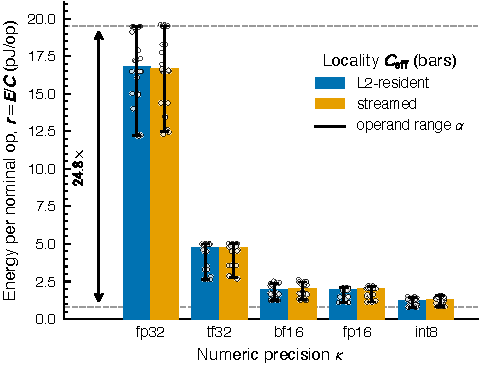
\includegraphics[width=\columnwidth]{exchange_band}
	\caption{The exchange-rate band of \cref{eq:betabare} (Experiment~1).
	Total energy quotient $E/C$ for a fixed matmul kernel on an NVIDIA
	A100, swept factorially over precision $\kappa$, operand locality
	$C_{\mathrm{eff}}$ (paired bars), and operand distribution $\alpha$;
	white points are the individual measured windows ($n=240$ across $60$
	cells). Dashed lines mark the band edges: the dearest cell is the band
	ceiling $r_{\mathrm{hi}}$, the cheapest (int8, zero operands) the
	envelope floor $r_{\mathrm{lo}}$.}
	\label{fig:exchange-band}
\end{figure}

\paragraph{Experiment 1---the exchange-rate envelope.}
A compute-bound matmul (operation count $C = 2MNK$ known analytically;
the int8 cells retire integer multiply--adds, counted as nominal operations
per the convention of \cref{subsec:forward}),
swept factorially over precision ($\kappa$, fp32 down to int8), operand
locality ($C_{\mathrm{eff}}$, operands resident in vs.\ streamed through
the L2 at a byte-identical shape), and operand
distribution ($\alpha$, zeros through adversarial-toggle), stratified by the
governor-selected clock. The pooled envelope spans
$r_{\mathrm{lo}} = 0.786$\,pJ/op (int8, zero operands) to
$r_{\mathrm{hi}} = 19.5$\,pJ/op (fp32), a span of $24.8\times$
(\cref{fig:exchange-band}), with precision following the textbook ordering
int8 $<$ bf16 $\approx$ fp16 $<$ tf32 $<$ fp32. Precision drives most of
the spread; operand values contribute a further factor ${\approx}2$ within
each format, and locality moves $r$ little for this compute-bound kernel.
The pooled span is descriptive of the hardware's full range; the floor
never reads it, because its two edges live in different formats. The
jointly feasible declared band for the fp16 case study is the fp16 cells'
own band, $[1.10,\,2.19]$\,pJ/op---a span of $2.0\times$, set by operands
and DVFS with the precision factor held fixed.

\begin{figure}[t]
	\centering
	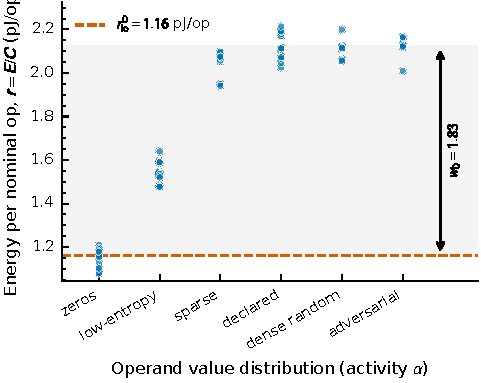
\includegraphics[width=\columnwidth]{operand_envelope}
	\caption{The operand envelope (Experiment~2, $n=96$ windows across six
	operand distributions). Kernel, shape, and precision (fp16) are held
	fixed and only the operand values vary; the SM clock was
	governor-selected, not locked, so the families do not share a common
	clock stratum (\cref{sec:empirical-measurements}). The figure is a
	descriptive within-device map of how far operand activity alone
	stretches $r$, not a clean isolation of the activity factor $\alpha$.
	The shaded span is the observed operand spread $w_0 = 1.83$; the
	minimum (zeros, dashed) is the descriptive fp16 operand floor,
	$1.16$\,pJ/op as a total quotient.}
	\label{fig:operand-envelope}
\end{figure}

\paragraph{Experiment 2---the operand-driven spread of $r$.}
The same matmul at fixed kernel, shape, and precision (fp16), now varying
only the operand \emph{values} (zeros, structured sparsity, low-entropy,
declared-typical, dense-random, adversarial maximum-toggle). The SM clock,
however, was governor-selected rather than locked (locking is
privilege-denied; \cref{sec:empirical-measurements}), and the operand
families did not run at a common clock---the cheapest (zeros, low-entropy)
drew the highest clocks and the dearest (dense-random, adversarial-toggle)
the lowest. This experiment therefore does not cleanly isolate the activity
factor $\alpha$; we read it as descriptive within-device evidence of the
operand-driven spread of $r$, not as a certified population edge. Operand
values alone spread $r$ by an observed factor $w_0 = 1.83$
(\cref{fig:operand-envelope}), following the ordering zeros $<$ low-entropy
$<$ structured-sparse $<$ dense-random $\approx$ adversarial-toggle
(\cref{app:operands} constructs the distributions explicitly). The clock
confound plausibly \emph{compresses} this spread rather than inflating
it---the cheap families ran fastest, so a common clock would, if anything,
spread the energies further---but we offer this only as a direction-of-bias
note, not a proof: DVFS voltage scaling, throughput, and baseline-power
amortisation pull in competing directions, and one-sided uncertainty cannot
repair an uncontrolled confound. No security bound rests on $w_0$ or on this
operand edge. The minimum-energy run (zeros) puts the fp16 operand floor at
$1.16$\,pJ/op as a total quotient---a descriptive edge only; the covert
denominator the floor actually uses is Experiment~7's marginal cost (a
one-sided $95\%$ lower confidence limit), which strips the baseline power
this quotient amortises in.

\begin{figure}[t]
	\centering
	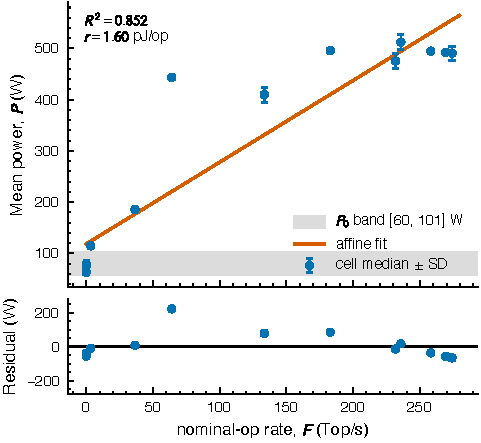
\includegraphics[width=\columnwidth]{overhead_affine}
	\caption{The overhead band and the affine forward map (Experiment~3,
	$n=65$ windows across a $15$-cell rate ladder). \emph{Top:} mean power
	$P$ vs.\ nominal-op rate $F$, plotted as per-cell medians with
	$\pm1$\,SD error bars over each cell's repeats, against the affine fit
	$P = rF + P_0$ ($R^2 = 0.852$; slope $r = 1.60$\,pJ/op); the shaded band
	is the observed idle range across five idle variants,
	$P_0 \in [59.8, 101.0]$\,W. \emph{Bottom:} residuals; the
	launch- and bandwidth-bound mid-ladder shapes carry the scatter. This is a
	\emph{between-shape} diagnostic of the affine map; the covert denominator
	the floor actually uses is the \emph{within-cell} marginal cost of
	\cref{fig:marginal-dose} (Experiment~7), not this fit.}
	\label{fig:overhead-affine}
\end{figure}

\paragraph{Experiment 3---the overhead band $\Delta E_0$ and the marginal rate.}
Sweeping the sustained operation rate from idle to saturation---five idle
variants (with and without a CUDA context, cached, cooled, post-load) and a
ten-shape matmul ladder---and fitting $P = rF + P_0$ of
\cref{eq:forward}. The observed idle range, widened by the meter's stated
$\pm 5\%$ tolerance, pins the overhead band to
$P_0 \in [59.8, 101.0]$\,W (width $\Delta P_0 = 41.2$\,W). The affine fit
across the full ladder gives a workload-averaged marginal rate of
$1.60$\,pJ/op with $R^2 = 0.852$ (\cref{fig:overhead-affine}): the map is
affine where the kernels are compute-bound, and the launch- and
bandwidth-bound mid-ladder shapes carry the residual scatter---heterogeneity
we report rather than prune away. As a sensitivity check, restricting the
fit to the idle anchors and the five compute-bound cubes gives
$1.65$\,pJ/op ($R^2 = 0.99$), within $4\%$ of the full-ladder slope; the
mid-ladder shapes account for the scatter, not the slope. This
between-shape slope is a diagnostic of the affine forward model, not the
floor's covert denominator: it averages over shapes whose non-covert
factors vary together, where the theorem needs the derivative at fixed
declared work. That derivative is what Experiment~7 identifies.

\begin{figure}[t]
	\centering
	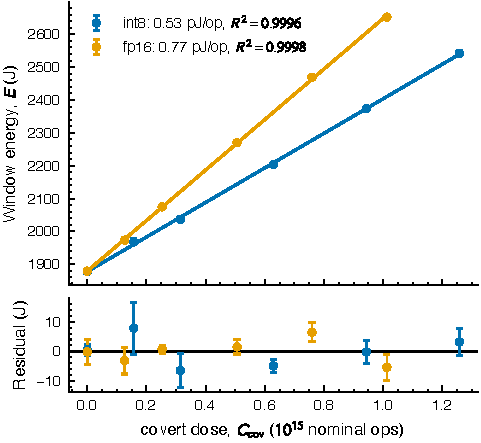
\includegraphics[width=\columnwidth]{marginal_dose}
	\caption{The marginal covert cost (Experiment~7): window energy $E$ vs.\
	covert dose $C_{\mathrm{cov}}$ for int8 and fp16 covert work, added to a
	fixed fp16 declared burst inside a fixed $10$\,s window. \emph{Top:}
	per-cell medians with $\pm1$\,SD error bars over the five repeats,
	against the dose fit $E = r_{\mathrm{cov}}\,C_{\mathrm{cov}} + E_0$; both
	slopes are linear to $R^2 > 0.999$ ($0.53$\,pJ/op int8, $0.77$\,pJ/op
	fp16) and share a zero-dose intercept matching the directly measured
	zero-dose windows to $0.02\%$. \emph{Bottom:} residuals. Because the
	baseline burns identically at every dose, it cancels in the slope: unlike
	the between-shape fit of \cref{fig:overhead-affine}, this within-cell
	slope is the incremental estimand $\partial E/\partial C_{\mathrm{cov}}$
	the floor's covert denominator requires (\cref{rmk:incremental}).}
	\label{fig:marginal-dose}
\end{figure}

\paragraph{Experiment 7---the marginal covert cost.}
The covert denominator, measured as the theorem defines it: the energy an
\emph{added} covert operation costs, with everything else held fixed. Every
measured window has the same fixed $10$\,s wall length and contains the
same calibrated fp16 declared burst (utilisation $0.30$ of the window,
declared-typical operands); to it we add $N_{\mathrm{cov}}$ covert matmuls
of one format (int8 or fp16, zero operands---the adversary's cheapest
case), then idle-pad to the window. Sweeping the covert dose over six
levels from zero to a $0.48$ busy fraction (randomised order,
drift-reference splices, five repeats per cell) and regressing window
energy on covert nominal operations gives the marginal cost as a slope
(\cref{fig:marginal-dose}):
$0.53$\,pJ/op for int8 and $0.77$\,pJ/op for fp16, both fits linear to
$R^2 > 0.999$, with the fitted zero-dose intercept agreeing with the
directly measured zero-dose windows to $0.02\%$. Because the fixed window
burns the same baseline energy at every dose, baseline power cancels in
the slope by construction---the marginal cost sits $0.26$ (int8) to
$0.39$\,pJ/op (fp16) below the corresponding total quotients, which
amortise it in. The floor
uses the one-sided $95\%$ \emph{lower} confidence limits,
$r_{\mathrm{lo}}^{\mathrm{cov}} = 0.51$\,pJ/op (int8) and $0.76$\,pJ/op
(fp16): the covert cost divides the slack, so under-pricing covert work
is the security-safe direction. Clock locking is denied on this platform,
so the governor is a recorded, not controlled, axis here too; the
window-median clock varies with the dose through the idle-pad share, and
the identification rests on the dose-response linearity and the intercept
anchor rather than on a common clock stratum---a stated limitation of the
platform.

\paragraph{Experiment 8---the marginal \emph{useful} covert cost.}
The same intervention, with the covert dose replaced by forward passes of the
trained-weight int8 transformer block of \cref{sec:decreasing-beta} (one
Pythia-6.9B layer on real text activations, quantisation scales applied, the
int8 matmuls and fp16 attention alike counted), swept at two shapes that
bracket the attention share of the op count. Regressing window energy on
covert nominal operations gives a marginal useful cost of $2.54$--$3.21$\,pJ/op
(both fits $R^2 > 0.999$; one-sided $95\%$ lower limits $[2.53, 3.16]$\,pJ/op),
against a standalone total quotient of $[3.18, 4.22]$: exactly as in
Experiment~7 the amortised idle baseline cancels in the slope, so this is the
incremental estimand the useful rungs of \cref{sec:decreasing-beta} require,
not a total quotient.

\paragraph{Assembling the floor.}
The floor is evaluated inside the jointly feasible fp16-declared scenario
of \cref{subsec:forward}: the declared band is the fp16 cells' own
$[r_{\mathrm{lo}}^{\mathrm{dec}}, r_{\mathrm{hi}}^{\mathrm{dec}}] =
[1.10,\,2.19]$\,pJ/op (Experiment~1), the covert cost is Experiment~7's
marginal lower limit, the overhead width is $\Delta P_0 = 41.2$\,W
(Experiment~3), and capacity and $\gamma$ come from the two formats'
published peaks. The set is format-consistent by construction---our
analysis code rejects any cross-format combination of extrema---and joint
attainability of its cheating corner within one observation window is
\cref{ass:corners}. Reading the fp16 cells as the declared band carries
one further disclosed assumption: that the declared work is executed in
its declared format. No off-site check enforces this; dropping it removes
the format pin entirely, so both declared edges open to the full hardware
envelope and the worst case rises to
$1.91$ (the bare-meter rung of \cref{sec:decreasing-beta}). With
covert int8 ($\gamma = 2$,
$r_{\mathrm{lo}}^{\mathrm{cov}} = 0.51$\,pJ/op) the energy-slack index at
full declared utilisation is
\begin{equation}
	S(1) \;=\; \mathbf{2.39},
	\label{eq:betameasured}
\end{equation}
or $1.62$ with covert work held to fp16
($r_{\mathrm{lo}}^{\mathrm{cov}} = 0.76$\,pJ/op). $S(1)$ is an
energy-only diagnostic, not a physical floor: at full declared
utilisation the capacity clip $(1-h)\gamma$ is zero, so no covert work
fits and $\beta_{\mathrm{phys}}(1) = 0$. The floor couples the slack to
that clip through \cref{eq:betaphys}. \Cref{fig:betaphys} traces
$\beta_{\mathrm{phys}}(h)$ for the two covert scenarios: with covert int8
against declared fp16 the worst case over utilisation is
\begin{equation}
	\beta_{\mathrm{phys}}^{*} \;=\; \mathbf{1.16}
	\quad\text{at}\quad h^{*} = 0.42,
	\label{eq:betaphysmeasured}
\end{equation}
and with covert work held to fp16 ($\gamma = 1$) it is $0.66$ at
$h^{*} = 0.34$. Energy is the binding constraint below the crossing,
capacity above it, and both bind at $h^{*}$: the worst case sits at
intermediate utilisation, where the declared work offers real cover but
still leaves much of the machine free.

This peak is a model \emph{upper} bound, and one that no single
observation window realises: $h^{*} = 0.42$ lies above the busy-time
ceiling $h_{\max} \approx 0.24$ (\cref{ass:corners}), so at the headline
utilisation the wall-clock budget binds before any schedule reaches the
corner. Restricting the maximisation to the utilisations our witness
construction can hold ($h \le h_{\max}$) puts the model worst case at
$\beta_{\mathrm{phys}} \approx 0.77$. We stress that $h_{\max}$ is a property
of that construction rather than a general feasibility bound: it is set by
this kernel's achieved rates and covert dose ratio, and includes a $10\%$
protocol margin so the idle pad never underflows (without it,
$h_{\max} = 0.27$ and the restricted worst case is $0.82$). A different
covert workload would move it. What we \emph{attain} is smaller
and measured directly: the matched-energy witnesses of
\cref{ass:corners} reach $h \approx 0.22$, where an accepted
cheating run hides $\mathbf{0.41}$ machines of covert int8 work. The
identified-set width the meter admits is therefore \emph{at least} $0.41$
machines---measured, attained, and accepted by the sensor---and
\emph{at most} about $1.16$ as a model bound whose maximiser is
infeasible, or about $0.77$ if the bound is confined to a feasible
window. Four-tenths of a machine of covert compute passing an honest
declaration is a wide identified set for a bare power meter; whether it
crosses the whole-machine ``vacuity'' line is not something the attained
witness settles, and we do not claim it does. The width is set jointly by
the energy budget and the silicon, not by either alone.

\begin{figure}[t]
	\centering
	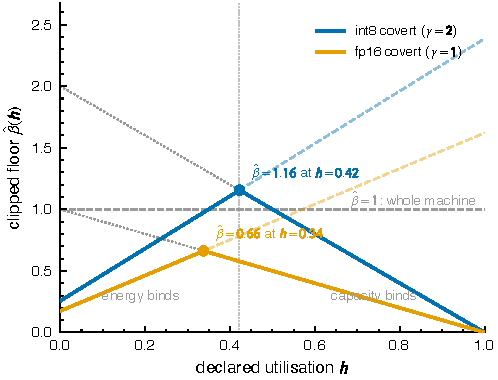
\includegraphics[width=\columnwidth]{beta_phys_curve}
	\caption{The capacity-clipped floor $\beta_{\mathrm{phys}}(h)$
	(\cref{eq:betaphys}) from the jointly feasible fp16-declared bands,
	for covert int8 ($\gamma = 2$, blue) and covert fp16 ($\gamma = 1$,
	orange), both priced at Experiment~7's marginal lower limits. Faint
	dashed lines are the unclipped energy-slack indices $S(h)$
	($S(1) = 2.39$ and $1.62$): energy is the binding constraint left of
	each crossing, capacity right of it, and both bind at $h^{*}$. Dotted
	lines are the capacity clips $(1-h)\,\gamma$; markers are the worst
	cases of \cref{eq:betaphysworst}.}
	\label{fig:betaphys}
\end{figure}

\section{The capability ladder}
\label{sec:decreasing-beta}

The bare meter is the worst case: the verifier sees nothing but the power,
and the prover has maximum wiggle room. Each capability the verifier gains
moves one band edge and shrinks the identified set by a measurable factor.
\Cref{tab:ladder,fig:ladder} walk down that ladder \emph{cumulatively}:
each rung adds one capability to all the rungs above it, and every priced
rung is recomputed as the same quantity the headline uses --- the
capacity-clipped physical worst case
$\beta_{\mathrm{phys}}^{*} = \max_h \beta_{\mathrm{phys}}(h)$ of
\cref{eq:betaphysworst}, under the joint model of
\cref{subsec:proposition}: fp16-declared case study, covert work priced at
the int8 marginal lower confidence limit $0.51$\,pJ/op
(\cref{sec:empirical-measurements}), $\gamma = 2$. The energy-slack
diagnostic $S(1)$ is reported alongside for orientation only: it is the
unclipped no-alarm budget at full utilisation, not a physical floor
($\beta_{\mathrm{phys}}(1) = 0$ --- a fully busy machine has no residual
capacity to hide work in). Because a verifier that gains a capability can
only shrink the set, the priced chain is monotone by construction, and a
regression test in the released code enforces it. Two disclosed
conditions thread the chain, marked $\dagger$ in \cref{fig:ladder} and
listed per rung in \cref{tab:ladder}: \emph{declared-format execution}
(from the precision rung down) and an \emph{observed operating point}
(from the re-execution rung down). The rest of this section takes the
rungs in turn.

\begin{table}[t]
	\centering
	\small
	\setlength{\tabcolsep}{3.5pt}
	\begin{tabular}{@{}lclcc@{}}
		\toprule
		verifier gains & type & band edge moved & $\beta_{\mathrm{phys}}^{*}$ & $S(1)$ \\
		\midrule
		nothing (bare meter) & --- & full envelope & $1.91$ & $37$ \\
		precision declared \& checked$^{\dagger}$ & D,\,C & $r^{\mathrm{dec}} \to [1.10, 2.19]$ & $1.16$ & $2.4$ \\
		clock \& locality observed & T & \emph{unpriced (prospective)} & --- & --- \\
		declared work re-executed$^{\ddagger}$ & C & $r_{\mathrm{hi}}^{\mathrm{dec}} - r_{\mathrm{lo}}^{\mathrm{dec}} \to$ gap & $0.34$ & $0.35$ \\
		covert work on useful data$^{\ddagger}$ & M & $r_{\mathrm{lo}}^{\mathrm{cov}}: 0.51 \to 2.53$ & $0.071$ & $0.072$ \\
		\emph{covert at top of useful band}$^{\ddagger}$ & A & $r_{\mathrm{lo}}^{\mathrm{cov}} \to 3.16$ & $0.057$ & $0.058$ \\
		\bottomrule
	\end{tabular}
	\caption{The capability ladder. Each rung grants the verifier one more
	capability (cumulative, top to bottom) and is re-priced as the clipped
	physical worst case
	$\beta_{\mathrm{phys}}^{*} = \max_h \beta_{\mathrm{phys}}(h)$
	(\cref{eq:betaphysworst}) under the joint model (fp16-declared case
	study, int8 covert edge at the Exp.~7 marginal LCB, $\gamma = 2$);
	$S(1)$ is the energy-only diagnostic, not a floor. Numeric band edges
	in pJ/op. Disclosed conditions: $\dagger$ --- assumes the declared work
	is executed in its declared format (an off-site check cannot enforce
	this; \cref{sec:decreasing-beta}); $\ddagger$ --- additionally assumes
	re-execution transfers at an observed operating point. Both are
	inherited by every rung below their first appearance. The type column
	says what kind of thing each rung is: D --- a declaration by the
	prover, checked off-site; C --- offline characterisation on the
	verifier's own hardware, transferring to the facility only up to a
	stated gap; T --- a trusted on-site observable, here left
	\emph{unpriced}: attested telemetry does not yet exist, and the
	measured operand spread $w_0$ is descriptive evidence, not a
	certified bound; M --- a threat-model restriction (hidden zero-ops
	are no threat); A --- an assumption about the adversary's objective,
	not a capability.}
	\label{tab:ladder}
\end{table}

\begin{figure}[t]
	\centering
	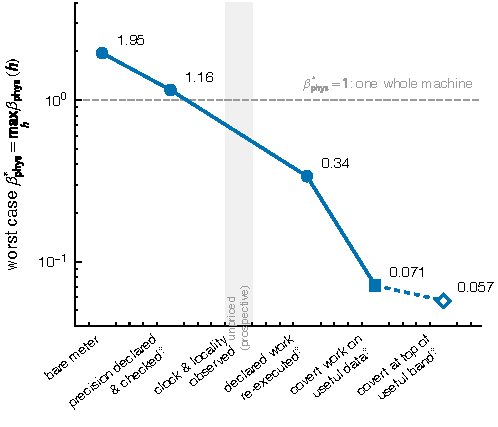
\includegraphics[width=\linewidth]{capability_ladder}
	\caption{The capability ladder of \cref{tab:ladder} on a log scale;
	every plotted value is the clipped worst case
	$\beta_{\mathrm{phys}}^{*} = \max_h \beta_{\mathrm{phys}}(h)$.
	Filled circles are verifier capabilities (types D, C); the square
	rung is forced by the threat model (type M: hidden zero-ops are no
	threat); the hollow rung is an assumption about the adversary, not a
	capability (type A). The shaded slot is the unpriced prospective
	clock/locality rung; daggered labels carry the disclosed conditions
	of \cref{tab:ladder}. The $\beta_{\mathrm{phys}}^{*} = 1$ line marks one
	whole machine of conceded ambiguity; the top two rungs are model upper
	bounds whose maximisers lie above the feasible window, so where they fall
	relative to that line is not something we claim to settle.}
	\label{fig:ladder}
\end{figure}

\paragraph{The bare meter ($\beta_{\mathrm{phys}}^{*} = 1.91$).}
With power alone the verifier cannot tell declared work from covert, nor one
numeric format from another, so both band edges are the full hardware
envelope of \cref{subsec:poweronly}: the honest acceptance ceiling is the
dearest measured rate ($r_{\mathrm{hi}} = 19.5$\,pJ/op, fp32) and the covert
floor is the cheapest incremental operation the silicon admits (the int8
marginal edge, $0.51$\,pJ/op). No precision is assumed on either side ---
reading the ceiling as the fp16 cell while opening the floor to int8 would
assume the declared format on one edge and deny it on the other, which a bare
meter cannot do. The resulting exchange span is $37.9\times$ --- wider than the
$24.8\times$ measured envelope, because the covert floor here is the int8
\emph{marginal} edge rather than the dearest-to-cheapest ratio of total
quotients --- wide enough that the capacity clip binds even at low utilisation:
the clipped
worst case peaks at $\beta_{\mathrm{phys}}^{*} = 1.91$ near
$h^{*} = 0.045$, essentially the int8 density advantage $\gamma = 2$ that a
near-idle machine leaves free. This maximiser sits \emph{inside} the
feasible window ($h^{*} < h_{\max} \approx 0.24$), so --- unlike the
precision rung, whose peak is pushed above the busy-time ceiling ---
confining the worst case to feasible utilisation does not lower it; the
bare-meter figure rests only on the corner assumption \cref{ass:corners}.
One consequence of the marginal covert pricing is worth flagging: the
overhead term $\Delta P_0 / (r_{\mathrm{lo}}^{\mathrm{cov}} F_{\mathrm{max}})
\approx 0.26$ has risen by half relative to a total-energy covert
quotient ($0.168 \to 0.259$), because the covert cost per operation it
divides by fell by a third ($0.786 \to 0.515$\,pJ/op).

\paragraph{Declare and check the precision ($1.91 \to 1.16$, conditional).}
The prover can be made to declare the declared work's numeric format, and
the verifier can re-run that work on its trusted cluster and confirm the
outputs are what fp16 execution produces. In the taxonomy of
\cref{tab:ladder} this rung is a declaration plus an offline check:
nothing new is sensed at the facility --- and that is exactly its limit.
The check makes the declaration \emph{precise}; it cannot make it
\emph{enforced}. What the rung buys, collapsing both declared edges from the
full hardware envelope to the fp16 band's own $[1.10, 2.19]$\,pJ/op (the
ceiling down from the fp32 rate $19.5$, the floor up from the int8 marginal
edge $0.51$), it buys only under the disclosed condition that
the declared work is actually executed in its declared format at the
monitored facility ($\dagger$ in \cref{tab:ladder}); facility-local format
enforcement is an open capability, not one this rung grants. Under that
condition the rung is precisely the headline case:
$\beta_{\mathrm{phys}}^{*} = 1.16$ at $h^{*} = 0.42$
(\cref{eq:betaphysmeasured}). Here and below, ``the verifier knows the
precision'' always means the \emph{declared} precision. The covert work's
precision is unobservable---declaring it would make it not covert---so it
never enters the numerator; it resurfaces at the bottom rungs.

\paragraph{Observe the clock and locality (unpriced).}
Voltage/clock (DVFS, of order $1.5$) and locality (weak for a compute-bound
kernel) are hardware-wide observables the power meter does not measure;
pinning them via other channels would narrow what remains of the declared
band down to its operand core. We deliberately quote no number for this
rung, for two reasons. First, the capability is prospective on every
candidate route: attested clock telemetry (NVML reports the clocks, but
firmware-reported numbers count only over the tamper-resistant read path
that \cref{sec:intro} notes does not yet exist), locked clocks by policy,
or, in principle, the EM side channel---switching at $f$ radiates at $f$
and its harmonics, and magnetic emanations from a GPU's power delivery are
measurable in practice \citep{maia2022magnetic}, though clock-line
radiation itself has not been demonstrated---with the voltage then
following from the hardware's $V$--$f$ table. Second, the number the old
arithmetic would have used, the operand core $w_0 = 1.83$, is descriptive
within-device evidence: Experiment~2's workload families ran at different
achieved clocks (the confound is disclosed in
\cref{sec:empirical-measurements}), so $w_0$ is not a certified population
edge and does not price a guarantee. The rung stays in the ladder as the
slot a trusted on-site observable would fill --- and the next rung depends
on it. The locality half is speculative: per-rail metering (core vs.\ HBM
regulators) or interconnect telemetry might resolve it; fortunately
Experiment~1 found locality moves $r$ little for compute-bound work.

\paragraph{Re-execute the declared work ($1.16 \to 0.34$, conditional).}
Re-executing to \emph{measure} the declared work's actual energy per operation,
not merely confirm its format, squeezes
$r_{\mathrm{hi}}^{\mathrm{dec}} \to r_{\mathrm{lo}}^{\mathrm{dec}}$ and the
numerator collapses to a residual set by the \emph{hardware gap}:
re-execution runs on the verifier's trusted cluster, not the monitored
facility, and energy per operation is hardware-specific---different accelerators,
firmware, cooling, operating point---so the measured $r^{\mathrm{dec}}$
transfers only up to a gap. That gap, not zero, is the floor on how far
re-execution can pin the declared band. The cross-device spread we measured
on three A100s of the same SKU---$2$--$3\%$ on every band edge
(\cref{subsec:proposition})---is a lower flavour; across different
accelerators, firmware, and cooling the gap is larger and unmeasured. We
take the residual gap at a few per cent of the declared rate,
${\approx}0.05$\,pJ/op (an assumption informed by the same-SKU spread, not
a cross-hardware measurement), giving $\beta_{\mathrm{phys}}^{*} = 0.34$
at $h^{*} = 0.83$ --- at this depth the overhead band, not the declared
residual, carries most of the width. Read the rung as a sensitivity
analysis in the gap, not a measured bound: at the same-SKU spread itself
(gap $0.02$--$0.04$\,pJ/op) the rung reads $0.29$--$0.32$; at our stated
$0.05$\,pJ/op, $0.34$; a cross-vendor gap of $0.2$\,pJ/op would put it at
${\approx}0.54$. Measuring that gap --- the same declared workload
characterised across accelerator generations and vendors --- is the
experiment this rung waits on.

The rung also inherits a second condition ($\ddagger$ in
\cref{tab:ladder}): \emph{re-execution only pays at an observed operating
point}. Re-execution measures the declared work's energy per operation at
the \emph{verifier's} operating point; if the prover's clock state is
unobserved --- and the previous rung is exactly the one still unpriced ---
the prover may run the declared work anywhere on the DVFS curve, and the
transfer error is not the hardware gap but the full DVFS factor of
${\sim}1.5$. A verifier with only ``power and paperwork'' (the power meter
plus declarations and re-execution, but no on-site sensing) therefore
stalls at $\beta_{\mathrm{phys}}^{*} \approx 1$: re-executing the declared
work buys almost nothing that checking its precision had not already
bought.

\paragraph{Restrict covert work to useful data ($0.34 \to 0.071$).}
This rung is forced by the threat model rather than granted by a channel,
and the logic runs in steps. Covert work is unseeable \emph{by definition}:
no declaration reaches it, so its floor $r_{\mathrm{lo}}^{\mathrm{cov}}$ is
bounded only by the silicon --- the int8 marginal edge, $0.51$\,pJ/op. But
the cheapest operations on that edge are operand zeros, and zeros compute
nothing useful: hidden zero-ops are no threat. We therefore measured the
\emph{incremental} cost of useful covert work directly: an int8-quantised
transformer block built from one trained Pythia-6.9B layer, run on real text
activations (not synthetic patterns), with the quantisation scales applied
and every metered operation --- the int8 matmuls and the fp16 attention
alike --- counted. Sweeping that block as the covert dose inside the
Experiment-7 construction (a fixed declared burst and fixed window, so
baseline power cancels in the dose slope; \cref{rmk:incremental}) prices
genuinely useful covert work at a \emph{marginal}
$r_{\mathrm{useful}} = [2.53, 3.16]$\,pJ/op (one-sided $95\%$ lower limits;
the standalone total quotient $E/C$ is $[3.18, 4.22]$, dearer only because it
amortises idle power the covert work does not draw). Restricting the adversary
to work worth doing raises the covert edge to the bottom of that band,
$0.51 \to 2.53$\,pJ/op, while the declared-side residual stays at the
hardware gap --- the covert band's own width prices nothing on the
declared side --- and the rung drops to
$\beta_{\mathrm{phys}}^{*} = 0.071$: every slack joule now buys the
adversary ${\approx}4.9\times$ fewer useful operations than silicon-floor
accounting would concede. Because this edge is an incremental dose slope, not
a standalone total quotient, it is a genuine marginal lower bound on the
covert cost --- the estimand the denominator requires (\cref{rmk:incremental}),
measured the same way as the int8 covert edge rather than left as its flagged
exception.

\paragraph{Covert work at the top of the useful band ($0.071 \to 0.057$).}
The final rung is an assumption, not a capability. Only by assuming the
covert work forgoes all of its remaining freedom inside the useful band
and pays that band's ceiling,
$r_{\mathrm{lo}}^{\mathrm{cov}} \to 3.16$\,pJ/op, does the residual fall
to ${\approx}0.057$. A bound of that order --- covert compute at several
per cent of capacity --- exists only on this rung, conditional on an
assumption about the adversary's objective rather than on any measurement; the
distinction matters for the power-monitoring layers proposed in the
verification literature \citep{baker2025verifying}.

\section{Discussion}
\label{sec:discussion}

\paragraph{The meter is an anchor, not an instrument.}
The result reads pessimistic --- against a bare power meter a
matched-energy witness demonstrably hides four-tenths of a machine of
covert compute, and the model worst case runs higher still, to
$\beta_{\mathrm{phys}}^{*} = 1.91$ against a bare meter --- a figure that
rests on the joint feasibility of the band corners (\cref{ass:corners}) ---
but the ladder inverts the reading. The
meter's role in a verification regime is not to count operations by itself; it
is to be the one channel whose integrity needs no trust in the prover, the
anchor against which declarations, attested clocks, and re-execution are
checked. Power plus checked declarations reaches
$\beta_{\mathrm{phys}}^{*} \approx 1.2$; adding an observed operating
point and re-execution of the declared work reaches ${\approx}0.34$, and
restricting covert work to useful data ${\approx}0.071$ of capacity. Every
rung is a protocol requirement a treaty could stipulate, together with a
disclosed condition it rests on, and \cref{eq:betaphysworst} states
exactly which band each requirement moves and by how much. The negative
result is equally operational: because re-execution transfers only at the
verifier's operating point, ``power plus paperwork'' --- declarations and
re-execution with no on-site sensing --- stalls at
$\beta_{\mathrm{phys}}^{*} \approx 1$, a regime design worth ruling out
before it is proposed.

\paragraph{What no verifier capability reaches.}
The denominator of \cref{eq:beta} is a statement about the adversary, not
the instrumentation. Covert work is by definition undeclared, so its
exchange rate is bounded only by the silicon and by what the threat model
says the adversary wants: excluding zero operands (which compute nothing)
raises the covert floor from the int8 marginal edge to the cheapest
\emph{useful} rate --- a measured $4.9\times$ step, $0.51$ to
$2.53$\,pJ/op --- and the remaining $1.25\times$, the useful band's own
width, closes only by assuming the adversary declines cheap-but-useful
work --- sparse activations, quantised weights --- that our own
measurements show exists. Any bound quoted for power-based verification
should state which side of that assumption it stands on.

\paragraph{From one device to a facility.}
Our bands are device physics, measured on one A100; a facility is a sum of
devices behind shared power delivery and cooling, and we deliberately do
not offer a fleet-average version of \cref{eq:beta}. Scaling the floor up
is a \emph{multi-resource allocation problem}, not a change of units: each
device carries its own capacity clip and utilisation, the prover chooses
how declared work is spread across devices (and formats) to maximise
cover, and the facility meter adds cooling and conversion overheads that
the prover partially controls. The identified set is then the projection
of a per-device product of constraints, and its width depends on the
allocation the prover is free to pick; treating $h$ as a single fleet
average can under- or overstate it. What does carry over qualitatively:
overhead bands widen at facility scale, and new datapaths (FP8, FP4)
widen the precision envelope beyond our $24.8\times$ and raise the
capacity ratio $\gamma$ of the cheapest format. Making the multi-device
floor precise---including which per-device telemetry restores the
single-device analysis---is open.

\paragraph{Limitations.}
Seven caveats bound the claims. (i) The bands come from one vendor, one
GPU model, one driver, and one cluster; the ladder's numbers are
A100-specific, though the closed form is not.
(ii) The band edges are read from a factorial sweep whose corner cell
(int8, zero operands) is directly measured, but on synthetic operands;
genuinely useful covert work prices at the measured marginal useful band
$[2.53, 3.16]$\,pJ/op instead (Experiment~8's dose-response; the standalone
total quotient is $[3.18, 4.22]$), and the bottom rungs depend on that band's
width. (iii) The hardware gap behind the
re-execution rung (${\approx}0.05$\,pJ/op) is an assumption. The same-SKU
piece is now grounded---band edges agree to $2$--$3\%$ across three A100s
(\cref{subsec:proposition})---but the cross-hardware gap (different
accelerators, firmware, cooling) remains unmeasured. (iv) DVFS was never
swept --- the platform denied clock-locking --- so the voltage factor
rides on literature numbers rather than our own; persistence mode was
likewise fixed on, so its contribution to the controllable idle range
went unmeasured. (v) Energy was read from on-die telemetry (a $10$\,Hz
zero-order hold with stated $\pm 5\%$ accuracy) in a non-adversarial lab
characterisation (\cref{sec:empirical-measurements});
an off-chip meter would add its own calibration band, which only widens
$\beta$. (vi) On shared nodes, windows stalled by co-tenants were dropped
by a pre-specified power guard, and high-tail windows are flagged rather
than deleted; all raw rows remain on disk. This flag-not-delete rule gates
only the \emph{descriptive} band medians (the pooled envelope, the operand
spread $w_0$). The quantities that actually enter the bound are of three
kinds, and we state the status of each rather than claim one statistical
coverage guarantee over all of them. (a) The covert denominator---the one
quantity a lower bound is genuinely sensitive to---is a one-sided $95\%$ lower
confidence limit on a regression slope (Experiments~3 and~7, and the
useful-band dose slope), coverage-controlled by construction. (b) The declared
band $[r_{\mathrm{lo}}^{\mathrm{dec}}, r_{\mathrm{hi}}^{\mathrm{dec}}]$ enters
only as a \emph{difference} of per-cell-median edges at a common saturated rate
(\cref{rmk:incremental}), so the amortised baseline cancels and it acts as a
band \emph{width}, not a point estimate needing its own coverage; its target
population is the achievable per-shape operating points of the declared format
on the audited A100 SKU, and the edges are that observed operating envelope.
(c) The overhead width $\Delta P_0$ and the capacity/$\gamma$ inputs are
conservative worst-case \emph{design} parameters, not sampled estimates:
$\Delta P_0$ is the observed idle envelope stretched by the meter's stated
$\pm 5\%$ tolerance (widening it only widens $\beta$), and $C_{\max}$ and
$\gamma$ are published hardware peaks. We therefore do not claim simultaneous
statistical coverage over the rectangle these edges span; the rectangle is a
deliberately conservative over-approximation, as no single schedule attains its
combined extrema (\cref{ass:corners}). (vii) The locality contrast is
attenuated in the fp32/tf32 cache-resident cells, whose operands
marginally spill L2.

\paragraph{What richer telemetry adds.}
Everything here is time-integrated, and the sufficiency of total energy
for a question about totals is a consequence of our \emph{free-variation}
model: because $r(t)$ and $P_0(t)$ may vary arbitrarily within their
bands, the trace's shape carries no information about totals beyond its
integral. Real hardware is not perfectly free---power-ramp limits, DVFS
governor dynamics, the instantaneous clip $F(t) \le F_{\max}$, and any
\emph{declared schedule} the prover commits to all constrain how the trace
can move, and a verifier who models them can extract more from the
resolved trace than from its integral. Conditional on the free-variation
model, then, the time \emph{profile} adds nothing about how much compute
ran; unconditionally, that is an open modelling question, not a theorem.
The profile also carries different information --- workload cadence,
training-step periodicity --- that bears on what \emph{kind} of compute
ran rather than how much; that question needs different machinery and is
treated in separate work.

The same caveat applies beyond the time axis. Our result prices the
integrated-energy channel under free variation; a verifier with richer
instrumentation is outside the model. Multiple simultaneous channels
(per-rail power, electromagnetic, thermal), cryptographically
authenticated telemetry (the proof-of-learning and zero-knowledge
proof-of-training protocols of \cref{ass:declaration}), or independently
controlled measurements the prover cannot shape (locked clocks,
tamper-resistant attested counters) each carry constraints the integral
does not, and any of them may narrow the identified set below the widths
reported here. The impossibility we state is for total-energy sensing
under the free-variation threat model, not for analogue sensing in
general.

\section{Conclusion}
\label{sec:conclusion}

A bare power meter cannot count operations. The energy cost of an operation
is unknown and data-dependent---the hardware's full envelope spans a
measured $24.8\times$ on an A100 ($0.79$--$19.5$\,pJ/op), and even inside
one jointly feasible declared format the band and the marginal covert cost
leave an energy slack ($S(1) = 2.39$, \cref{eq:betameasured}, an
energy-only diagnostic since no covert work fits at full utilisation).
Coupling that slack to silicon capacity gives the clipped floor of
\cref{eq:betaphys}. What we \emph{attain} and the sensor accepts is a
matched-energy witness hiding $0.41$ machines of covert int8 work at
$h \approx 0.22$; the model worst case peaks higher,
$\beta_{\mathrm{phys}}^{*} = 1.16$ at $h^{*} = 0.42$
(\cref{eq:betaphysmeasured}, $1.91$ against the bare meter with the
declared format unenforced), but that peak is an upper bound whose
maximiser sits above the busy-time ceiling---confined to a feasible
window the model worst case for the precision-checked sensor is about $0.77$. The identified-set width the
meter admits is thus at least $0.41$ machines and at most about one, set
jointly by the energy budget and the silicon. This is not a statistical
shortfall a better meter or a longer window repairs; it is a structural
degeneracy of the integrated-energy forward map under free variation --- a
property of the model, not of the A100. The specific widths above (the
$24.8\times$ span, $S(1) = 2.39$, the measured $0.41$, and the model
$\beta_{\mathrm{phys}}^{*} = 1.16$/$1.91$) are contingent A100 estimates;
the closed form they instantiate is device-agnostic. An identified set
this wide---four-tenths of a machine of covert compute demonstrably
passing an honest declaration---substantially weakens the raw
joules-to-FLOPs conversion in the governance literature against an
adversary free to vary energy intensity.

But the floor is a closed form built from named physical bands, and that
is what makes it useful: each verifier capability moves one band edge by a
measured amount, and every rung is re-priced as the same clipped worst
case $\max_h \beta_{\mathrm{phys}}(h)$. Precision declared and checked
brings the worst case from $1.91$ to $1.16$, conditional on the declared
work executing in its declared format; re-execution of the declared work
at an observed operating point to ${\approx}0.34$ --- a residual that
rests on a stated hardware-gap assumption, not a measurement
(\cref{tab:ladder}). The rungs interlock --- re-execution pays only at an
observed operating point, so power plus paperwork stalls at
${\approx}1$ --- and no capability reaches the covert side: restricting
covert work to the measured useful-operand band brings ${\approx}0.071$,
and the final collapse to ${\approx}0.057$ closes only by assumption on
the adversary. This paper prices each rung, with its conditions stated,
so that a verification regime can be designed --- or rejected --- on
numbers rather than on the intuition that joules imply FLOPs.

\bibliography{references}
\bibliographystyle{icml2026}

\newpage
\appendix
% From here on, section-counter labels are appendices: make cleveref say
% "Appendix A" rather than "Section A". \crefalias is captured at \label time,
% so body-section references (defined earlier) are unaffected.
\crefalias{section}{appendix}
\crefname{appendix}{Appendix}{Appendices}
\Crefname{appendix}{Appendix}{Appendices}
\onecolumn

\section{From the CMOS power law to the exchange rate}
\label{app:cmos}

The back-of-the-envelope argument of \cref{subsec:envelope} adopts the
factored exchange-rate model \cref{eq:cmos}. We derive it here from the CMOS
power law \citep{chandrakasan1992lowpower} and locate the terms the
factorisation drops. Total chip power separates into a dynamic (switching)
part and a static part,
\begin{equation}
	P = P_{\mathrm{dyn}} + P_{\mathrm{stat}}, \qquad
	P_{\mathrm{dyn}} = \alpha\, C\, V^2 f, \qquad
	P_{\mathrm{stat}} = V I_{\mathrm{leak}} + P_{\mathrm{fixed}},
	\label{eq:powertotal}
\end{equation}
with $\alpha$ the activity factor, $C$ the switched capacitance, $V$ the
supply voltage, $f$ the clock, $V I_{\mathrm{leak}}$ the leakage power, and
$P_{\mathrm{fixed}}$ the cooling, I/O, and idle draw. The forward model
\cref{eq:forward}, $P = rF + P_0$, is slope--intercept in the operation rate $F$,
so the exchange rate is the \emph{marginal} energy per operation and the overhead
is the intercept,
\begin{equation}
	r = \frac{\partial P}{\partial F}, \qquad P_0 = P\big|_{F=0}.
	\label{eq:marginal}
\end{equation}
Experiment~3 estimates \cref{eq:marginal} directly, regressing mean power
on sustained nominal-op rate with idle cells as the $F = 0$ anchors
(\cref{sec:empirical-measurements}).

\paragraph{The dynamic term gives $r$.}
The operation rate is $F = N_{\mathrm{op}}\,f$, where $N_{\mathrm{op}}$ is
the number of nominal operations the datapath retires per cycle at the operating format
(an idle unit lowers the activity $\alpha$, not the clock $f$). At a fixed
format the clock is thus the knob through which the operation rate moves,
$\partial f/\partial F = 1/N_{\mathrm{op}}$, and the marginal rate of
\cref{eq:marginal} follows by the chain rule, holding $\alpha$, $C$, and $V$
fixed,
\begin{equation}
	r \;=\; \frac{\partial P_{\mathrm{dyn}}}{\partial F}
	\;=\; \frac{\partial P_{\mathrm{dyn}}}{\partial f}\,\frac{\partial f}{\partial F}
	\;=\; \frac{\alpha\, C\, V^2}{N_{\mathrm{op}}}
	\;=\; \alpha\,\Bigl(\tfrac{C}{N_{\mathrm{op}}}\Bigr)\,V^2 ,
	\label{eq:rdyn}
\end{equation}
and the clock drops out: energy per operation does not depend on how fast
the operations run, only on what each switching event costs and how many
operations it delivers. The rate is constant in $F$, so $P_{\mathrm{dyn}} = rF$
is linear through the origin, exactly the affine form the forward model
\cref{eq:forward} assumes and Experiment~3 fits. The capacitance switched
per operation, $C/N_{\mathrm{op}}$, has two structural sources: the arithmetic
datapath, whose width is set by the numeric format, and the data-movement
path, set by where the operands live and which kernel runs. Factoring it
accordingly,
\begin{equation}
	\frac{C}{N_{\mathrm{op}}} \;=\; \kappa(\text{precision})\;C_{\mathrm{eff}}(\text{locality},\,\text{kernel}),
	\label{eq:capfactor}
\end{equation}
with $\kappa$ collecting the format scale (datapath width and the operation
packing $N_{\mathrm{op}}$) and $C_{\mathrm{eff}}$ the locality and kernel
structure, and substituting into \cref{eq:rdyn}, gives the model
\cref{eq:cmos}. This is a re-parameterisation by physical origin, not a
unique factorisation: $\kappa$, $\alpha$, and $C_{\mathrm{eff}}$ are all
switching quantities, grouped by cause---format, operand data, memory
locality---so that each maps to a single verifier category.

\paragraph{Short-circuit sits in $r$, inside the switched capacitance.}
\citet{chandrakasan1992lowpower} also carry a \emph{short-circuit} term for
the direct-path current that flows while an input transitions and the NMOS
and PMOS networks briefly conduct together. It is triggered by the same
switching events as $P_{\mathrm{dyn}}$, so it scales with the operation rate and
survives the marginal derivative of \cref{eq:marginal}. In a well-designed
circuit it is a small fraction of the switching power, so we fold it into
the effective switched capacitance $C_{\mathrm{eff}}$ of \cref{eq:capfactor}:
it lands in $r$, but introduces no new verifier category.

\paragraph{Leakage sits in $P_0$, not $r$.}
The static power $P_{\mathrm{stat}}$ of \cref{eq:powertotal} flows whether
or not the machine computes, so
$\partial P_{\mathrm{stat}}/\partial F = 0$: by \cref{eq:marginal} it
contributes nothing to the marginal rate $r$ and is entirely the intercept
$P_0$, where the derivation of \cref{eq:integrated} already places it and
carries it as a bounded nuisance band. A leakage-per-operation term
$r_{\mathrm{leak}} = P_{\mathrm{stat}}/F$ would appear only if $r$ were
defined as the \emph{average} energy per operation, $P/F$, which mixes in the
intercept and is operating-point dependent; we keep the marginal definition
\cref{eq:marginal}, consistent with \cref{eq:forward}, and so carry no
separate leakage term in $r$.

\section{How Experiment~1 measures the exchange rate}
\label{app:bench}

Experiment~1 (\cref{sec:empirical-measurements}) reads the \emph{total
energy quotient} $E/C$ off a single A100 by holding the workload fixed and
moving one factor of \cref{eq:cmos} at a time. The quotient is the
band-edge estimand of \cref{sec:empirical-measurements}---not the marginal
rate $r = \partial P/\partial F$ of \cref{eq:forward}, which Experiments~3
and~7 estimate as regression slopes---and we keep the two apart throughout.
This appendix gives the mechanics: the workload and why its operation count
is exact, how each driver is set, and how the energy is metered.
Experiments~2 and~3 reuse the same protocol with a different swept axis;
Experiment~7 reuses its metering inside fixed-length composite windows
(declared burst + covert dose + idle pad).

\paragraph{The workload and its exact operation count.}
Every cell runs a dense square matrix multiply $A\,B$ with
$A\in\mathbb{R}^{M\times K}$, $B\in\mathbb{R}^{K\times N}$ (we take
$M=N=K=n$). Each of the $MN$ output entries is a dot product of length
$K$---$K$ multiplies and $K{-}1$ adds---so by the standard
two-operations-per-multiply-add convention the matmul costs
\begin{equation}
	C \;=\; 2MNK \;=\; 2n^3 \quad \text{op},
	\label{eq:flopcount}
\end{equation}
counted as nominal operations of whatever format the cell runs (int8
multiply--adds included; \cref{subsec:forward}),
known \emph{analytically} from the shapes alone, with no profiler or
hardware counter involved. A measured window runs \texttt{iters} such
matmuls back to back, so its nominal compute is
$C_{\mathrm{win}} = 2n^3\,\texttt{iters}$ and the energy per operation is
$r = E_{\mathrm{win}} / C_{\mathrm{win}}$. Because $C$ is exact, $r$
inherits the meter's accuracy directly; and because $r$ is intensive
(energy \emph{per} operation), cells of different size and \texttt{iters}
compare directly.

\paragraph{Setting the swept drivers.}
\begin{itemize}
	\item \textbf{Precision $\kappa$} is the tensor \texttt{dtype}:
	\texttt{fp32}, \texttt{tf32} (fp32 operands routed through the tf32
	tensor-core path), \texttt{fp16}, \texttt{bf16}, and \texttt{int8} (an
	integer-matmul kernel, int8$\times$int8$\to$int32). Lower precision
	charges less capacitance per multiply-accumulate, lowering $\kappa$.
	\item \textbf{Locality $C_{\mathrm{eff}}$} is operand \emph{residency}
	at a byte-identical shape, not problem size: sweeping it by changing $n$
	would change the operation count and confound the comparison, so instead
	we fix the shape at $n = 2048$ and vary how many distinct operand sets
	the window rotates through iteration to iteration. The A100 has a
	40\,MB L2; at $n = 2048$ an fp16 $A$--$B$ operand set is ${\sim}16$\,MB,
	so:
	\begin{itemize}
		\item \emph{resident} (one operand set, reused every iteration): the
		working set fits the L2, so most traffic is served on-chip and HBM
		activation is avoided: low $C_{\mathrm{eff}}$;
		\item \emph{streamed} (eight operand sets, round-robined): a reuse is
		evicted before it recurs, so every iteration streams fresh tiles from
		HBM, engaging its arrays, peripheral logic, and I/O: high
		$C_{\mathrm{eff}}$.
	\end{itemize}
	Both arms run the identical shape, kernel, and operation count
	\cref{eq:flopcount}; only the memory-traffic path differs, so locality no
	longer confounds the count. The kernel stays compute-bound in both
	arms---a $2048^3$ matmul is high arithmetic intensity---so streaming
	raises $C_{\mathrm{eff}}$ without making the workload memory-bound, and
	\cref{fig:exchange-band} accordingly shows locality moves $r$ only
	slightly.
\end{itemize}
The third driver, supply voltage $V^2$ (DVFS), we could not sweep: the
platform denied user clock-locking, so the clock was left to the governor
and merely recorded per run. The operand \emph{values} are a fourth axis:
Experiment~1 crosses all six operand distributions (\cref{app:operands})
with precision and locality in a full factorial, so the pooled envelope
already contains the operand spread; Experiment~2 re-runs the operand axis
alone, at fixed precision and locality, as the descriptive operand-only map
of \cref{app:operands}.

\paragraph{Metering the energy.}
Energy is read from the on-die NVML total-energy counter: the window energy
is one subtraction $E_1 - E_0$, with a \texttt{cuda.synchronize()} fence
bracketing each latch so the delta spans exactly the window's kernels;
where the counter is unavailable we integrate the power query in a
background sampler. Each cell fills a ${\sim}1.5$\,s window with matmuls
run back to back on pre-allocated buffers, with no host traffic inside the
window: long enough that counter quantisation is negligible, and saturated
enough that the joules are the datapath doing arithmetic, not allocation or
transfer. A few warm-up windows absorb JIT and clock ramp, several measured
windows follow, and the per-cell median is kept; shuffling the cell order
and periodically re-measuring a fixed reference cell guards against slow
thermal drift. The largest per-cell median over the sweep is the band
ceiling $r_{\mathrm{hi}}$; \cref{fig:exchange-band} plots the full set.

\section{How Experiment~2 varies the operands}
\label{app:operands}

Experiment~2 (\cref{sec:empirical-measurements}) holds the kernel, shape,
and precision fixed and moves \emph{only the operand values}; the SM clock
was governor-selected rather than locked (locking is privilege-denied), so
it is recorded per window and stratified in analysis, not held. Every
configuration runs the identical matmul $A\,B$ with the identical operation
count \cref{eq:flopcount}, so the energy differences track the
switching-activity factor $\alpha$ of \cref{eq:cmos}---how many bits
physically toggle in the datapath as the multiply--accumulates stream
through---though, because the clock was not controlled, we read the
resulting spread as descriptive rather than as a clean measurement of
$\alpha$ alone (\cref{sec:empirical-measurements}). A datapath that sees the
same bits over and over charges little capacitance; one whose bits flip on
every operation charges the most. The six distributions are constructed to
walk $\alpha$ from its floor to its ceiling. Below we show each on a
$4\times4$ patch; the real operands are the same patterns at full size,
generated by \texttt{operand\_fill} in \texttt{powertoflops/bench/workload.py}.

\paragraph{1. Zeros---the activity floor.}
Every entry is zero, so no bits ever change and $\alpha$ is at its minimum:
\begin{equation*}
	A_{\mathrm{zeros}} \;=\;
	\begin{pmatrix} 0 & 0 & 0 & 0 \\ 0 & 0 & 0 & 0 \\ 0 & 0 & 0 & 0 \\ 0 & 0 & 0 & 0 \end{pmatrix}.
\end{equation*}
This is the cheapest run at fixed fp16 and sets the descriptive fp16
operand floor, $1.16$\,pJ/op as a total quotient; combined with the int8
format in Experiment~1's factorial it reaches the full envelope floor
$r_{\mathrm{lo}} = 0.786$\,pJ/op. (The floor's covert denominator is
Experiment~7's marginal cost, not these quotients;
\cref{sec:empirical-measurements}.)

\paragraph{2. Low-entropy---a few distinct levels.}
Entries are drawn from only four values $\{0,1,2,3\}$. With so few distinct
bit patterns, few bits differ between neighbouring operands, so operand-bit
entropy---and hence switching---stays low:
\begin{equation*}
	A_{\mathrm{low\text{-}entropy}} \;=\;
	\begin{pmatrix} 1 & 0 & 3 & 1 \\ 2 & 2 & 0 & 3 \\ 0 & 1 & 1 & 2 \\ 3 & 0 & 2 & 1 \end{pmatrix}.
\end{equation*}

\paragraph{3. Structured-sparse---half the operands forced to zero.}
Dense random values, but a fixed half of the columns are deterministically
zeroed (every other column), giving exactly $50\%$ zeros in a regular
pattern: the structured sparsity real accelerators exploit, rather than
random dropout. The persistent zero columns roughly halve the switching
relative to a fully dense operand:
\begin{equation*}
	A_{\mathrm{sparse}} \;=\;
	\begin{pmatrix}
		0 & \phantom{-}0.4 & 0 & -0.9 \\
		0 & -0.7 & 0 & \phantom{-}0.2 \\
		0 & \phantom{-}0.8 & 0 & \phantom{-}0.5 \\
		0 & -0.3 & 0 & -0.6
	\end{pmatrix}.
\end{equation*}

\paragraph{4. Dense-random---generic busy data.}
Every entry is an independent uniform draw from $[-1,1]$: no zeros,
full-width mantissas, high but not maximal switching. This is the
realistic-workload reference:
\begin{equation*}
	A_{\mathrm{dense}} \;=\;
	\begin{pmatrix}
		\phantom{-}0.31 & -0.82 & \phantom{-}0.55 & -0.14 \\
		-0.67 & \phantom{-}0.09 & -0.48 & \phantom{-}0.73 \\
		\phantom{-}0.21 & \phantom{-}0.64 & -0.95 & \phantom{-}0.38 \\
		-0.52 & -0.27 & \phantom{-}0.86 & -0.41
	\end{pmatrix}.
\end{equation*}

\paragraph{5. Declared-typical---the realistic-activation stand-in.}
Every entry is an independent standard-normal draw, $\mathcal{N}(0,1)$: a
proxy for the activations and weights a genuine declared workload streams,
with full-width mantissas and no engineered structure. Its switching sits
alongside dense-random---high but not maximal---and it is the operand class
that characterises the honest-window energy scatter used by the declared-work
model:
\begin{equation*}
	A_{\mathrm{decl}} \;=\;
	\begin{pmatrix}
		\phantom{-}0.42 & -1.13 & \phantom{-}0.27 & -0.68 \\
		-0.35 & \phantom{-}0.91 & -1.42 & \phantom{-}0.11 \\
		\phantom{-}1.06 & -0.24 & \phantom{-}0.58 & -0.83 \\
		-0.72 & \phantom{-}0.39 & -0.16 & \phantom{-}1.24
	\end{pmatrix}.
\end{equation*}

\paragraph{6. Adversarial-toggle---the activity ceiling.}
Engineered for maximal switching: the matrix is a checkerboard of two
\emph{complementary} bit patterns, $\texttt{0x5555}\ldots$ and its bitwise
inverse $\texttt{0xAAAA}\ldots$, so adjacent operands differ in \emph{every}
bit (maximal Hamming distance) and the datapath flips as many transistors
as physically possible per operation. For floats the pattern is built in an
integer bit-view of the same width and reinterpreted as the float type, so
the raw bits---not the numeric value---are controlled exactly. Writing the
two patterns as $p$ and $\bar p$:
\begin{equation*}
	A_{\mathrm{adv}} \;=\;
	\begin{pmatrix}
		p & \bar p & p & \bar p \\
		\bar p & p & \bar p & p \\
		p & \bar p & p & \bar p \\
		\bar p & p & \bar p & p
	\end{pmatrix},
	\qquad
	p = \texttt{0x5555}\ldots,\;\; \bar p = \texttt{0xAAAA}\ldots
\end{equation*}
A matmul forms each output as a dot product
$\text{out}[i,j]=\sum_k A[i,k]\,B[k,j]$, streaming $k=0,1,2,\ldots$ and
loading one operand into the multiplier's input register each cycle.
Because every row and every column of the checkerboard alternates
$p,\bar p,p,\ldots$, that register walks
\begin{equation*}
	\underbrace{\mathtt{0101\,0101}}_{k=0}\;\to\;\underbrace{\mathtt{1010\,1010}}_{k=1}\;\to\;
	\underbrace{\mathtt{0101\,0101}}_{k=2}\;\to\;\cdots
\end{equation*}
flipping \emph{all} its bits on \emph{every} cycle. Dynamic CMOS energy is
paid per bit-transition, so this draws the most switching the datapath can
do: a $w$-bit operand toggles $w$ bits per cycle, against ${\approx}w/2$
for dense-random (two random words differ in about half their bits) and $0$
for zeros or any constant operand (the register never changes). The
checkerboard is simply the 2-D layout that makes the row sequence (feeding
$A$) and the column sequence (feeding $B$) both alternate this way at once,
for every output entry.

The energy-per-operation spread from the cheapest patch ($A_{\mathrm{zeros}}$)
to the densest operands (dense-random, declared-typical, and the adversarial
checkerboard), at fixed operation count, is the observed operand spread
$w_0 = 1.83$ of \cref{fig:operand-envelope}. The measured ordering follows
the textbook one, zeros $<$ low-entropy $<$ structured-sparse $<$
dense-random $\approx$ declared-typical $\approx$ adversarial-toggle. Because
the SM clock was governor-selected rather than locked
(\cref{sec:empirical-measurements}), this spread is descriptive within-device
evidence of how far operand activity can stretch the meter, not a clean
isolation of $\alpha$ and not a certified population edge; no security bound
in the paper rests on it.

\end{document}
